\documentclass[onecolumn,unpublished,a4paper]{quantumarticle}
\usepackage[utf8]{inputenc}
\usepackage[backend=biber,style=alphabetic,maxbibnames=999]{biblatex}
\usepackage{amsmath}
\usepackage{amssymb}
\usepackage{amsthm}
\usepackage{amsfonts}
\usepackage[caption=false]{subfig}
\usepackage[colorlinks]{hyperref}
\usepackage[all]{hypcap}
\usepackage{tikz}
\usepackage{relsize}
\usepackage{color,soul}
\usepackage{capt-of}
\usepackage{mathtools}
\usepackage{float}
\usepackage[section]{placeins}
\usepackage{listings}
\usepackage[T1]{fontenc}  % Without this, underscores lost when copy-pasting output!
\usetikzlibrary{decorations.pathreplacing}
\usepackage{braket}

\addbibresource{refs.bib}

\DeclareFixedFont{\ttb}{T1}{txtt}{bx}{n}{4}
\DeclareFixedFont{\ttm}{T1}{txtt}{m}{n}{4}
\definecolor{deepblue}{rgb}{0,0,0.5}
\definecolor{deepred}{rgb}{0.6,0,0}
\definecolor{deepgreen}{rgb}{0,0.5,0}
\newcommand\cppstyle{\lstset{
language=C++,
basicstyle=\ttm,
otherkeywords={uint8_t, __m256i, size_t, ASSERT_TRUE, EXPECT_TRUE, TEST, BENCHMARK},
keywordstyle=\ttb\color{deepblue},
emphstyle=\ttb\color{deepblue},
stringstyle=\color{deepgreen},
commentstyle=\fontfamily{txtt}\selectfont\color{gray},
showstringspaces=false,
literate={*}{{\char42}}1
         {-}{{\char45}}1
}}
\lstnewenvironment{cpp}[1][]
{\cppstyle\lstset{#1}}{}

\newcommand\pythonstyle{\lstset{
language=python,
basicstyle=\ttm,
morekeywords={assert,as,echo},
keywordstyle=\ttb\color{deepblue},
emphstyle=\ttb\color{deepblue},
stringstyle=\color{deepgreen},
commentstyle=\fontfamily{txtt}\selectfont\color{gray},
showstringspaces=false,
literate={*}{{\char42}}1
         {-}{{\char45}}1
}}
\lstnewenvironment{python}[1][]
{\pythonstyle\lstset{#1}}{}

\lstdefinestyle{stimcircuit}{
    language=python,
    basicstyle=\fontsize{6}{6}\selectfont\ttfamily,
    upquote=true,
    stepnumber=1,
    numbersep=8pt,
    showstringspaces=false,
    breaklines=true,
    frame=single,
    aboveskip=1.5em,
    belowskip=1.5em,
    commentstyle=\color{gray},
    classoffset=1,
    morekeywords={DETECTOR,OBSERVABLE_INCLUDE,rec},
    keywordstyle=\color{deepgreen},
    classoffset=2,
    morekeywords={H,R,MPP,M,RX,RY,MY,MX,SQRT\_X,XCY,XCZ,YCX},
    keywordstyle=\color{deepblue},
    classoffset=3,
    morekeywords={X_ERROR,DEPOLARIZE2,DEPOLARIZE1},
    keywordstyle=\color{red},
    classoffset=4,
    morekeywords={TICK,SHIFT_COORDS,QUBIT_COORDS},
    keywordstyle=\color{gray}
}

\hypersetup{linkcolor=blue}

% Boo Roman Numerals.
\renewcommand\thesection{\arabic{section}}

% Hyperlinked references to figures, theorems, etc.
\theoremstyle{definition}
\newtheorem{definition}{Definition}[section]
\theoremstyle{definition}
\newtheorem{theorem}[definition]{Theorem}
\theoremstyle{definition}
\newtheorem{lemma}[definition]{Lemma}
\newcommand{\eq}[1]{\hyperref[eq:#1]{Equation~\ref*{eq:#1}}}
\renewcommand{\sec}[1]{\hyperref[sec:#1]{Section~\ref*{sec:#1}}}
\DeclareRobustCommand{\app}[1]{\hyperref[app:#1]{Appendix~\ref*{app:#1}}}
\newcommand{\fig}[1]{\hyperref[fig:#1]{Figure~\ref*{fig:#1}}}
\newcommand{\tab}[1]{\hyperref[tab:#1]{Table~\ref*{tab:#1}}}
\newcommand{\theoremref}[1]{\hyperref[theorem:#1]{Theorem~\ref*{theorem:#1}}}
\newcommand{\definitionref}[1]{\hyperref[definition:#1]{Definition~\ref*{definition:#1}}}

\begin{document}
\title{Yoked Surface Codes: Denser Storage with one $Y^{\otimes n}$ Check}

\date{\today}
\author{Craig Gidney}
\email{craig.gidney@gmail.com}
\affiliation{Google Quantum AI, Santa Barbara, California 93117, USA}

\author{Michael Newman}
\affiliation{Google Quantum AI, Santa Barbara, California 93117, USA}

\author{Cody Jones}
\affiliation{Google Quantum AI, Santa Barbara, California 93117, USA}

\begin{abstract}
We improve the coding rate of surface codes by intermittently checking a logical $Y^{\otimes n}$ stabilizer (the ``yoke'').
When the yoke detects a problem, we use soft information from the execution history of the yoked surface codes to guess at a correction.
We show that yoked surface codes have 50\% better coding rates than normal surface codes, when targeting error rates below $10^{-9}$ per patch round starting from a gate error rate of $10^{-3}$.
Our estimates include the space and time overheads from the lattice surgery required to check the yokes, and our constructions make no additional demands of the hardware compared to normal surface codes.
Therefore, yoking represents a notable improvement in the expected cost of building large scale fault tolerant quantum computers.
\end{abstract}

\textbf{Data availability}: the code written, circuits generated, and stats collected for this paper are available on Zenodo at \href{https://doi.org/10.5281/zenodo.7901729}{doi.org/10.5281/zenodo.7901729}~\cite{gidneyhoneycombdata2022}[[[UPDATE LINK]]].

\maketitle

\tableofcontents

\section{Introduction}
\label{sec:introduction}

Because of its forgiving quality and connectivity requirements~\cite{fowler2012surfacecodereview}, the surface code is a leading contender for the error correcting code to use in the architecture of large scale fault tolerant quantum computers.
The surface code's major downside is its extremely demanding quantity requirements.
It takes 1000 to 2000 physical qubits per logical qubit for the surface code to reach error rates low enough to run classically intractable algorithms such as Shor's algorithm~\cite{shor1994,fowler2012surfacecodereview,gidney2021factor,soeken2020improved,litinskyhypercubeshor2023}.

There are many ideas in the field for improving coding rates~\cite{tremblay2022ldpc,higgott2021hyperbolic,bravyi2011subsystembacon,berthusen2023partialmeasure}[[[NEED MORE SUGGESTIONS HERE]]], as well as bounds on possible improvements~\cite{pattison2023planarcircuitbounds}[[[[NEED MORE SUGGESTIONS HERE]]]].
One type of idea is concatenating an error correcting code over the surface code.
In this idea, the underlying surface code suppresses noise below the threshold of the overlying code, and provides mechanisms such as lattice surgery~\cite{fowler2018latticesurgery,litinski2019gameofsurfacecodes} for performing operations between distant qubits.
The overlying code then suppresses the remaining noise down to the level required by the algorithm, hopefully with a final footprint lower than just using the surface code.

In the past, when we've tried to use this type of idea, we've usually imagined that the overlying code would be complicated.
We assumed the code would need a good mix of high distance and great coding rate in order to come out ahead.
Requiring these things together tends to demand complexity.
Using a complicated code is a problem for many reasons.
First, there's a lack of tooling, meaning each code you try requires substantial human effort to analyze.
For example, the layout of the lattice surgery measuring the stabilizers of the code has enormous implications on the code's viability when concatenated over the surface code.
Someone or something has to produce this layout and estimate how well it works.
Second, complicated codes have a tendency to be large and unwieldy, because the best numbers are in the asymptotic limit.
For example, in a complicated code, performing a single operation involving an encoded qubit may require touching dozens or hundreds of surface code patches that are spread across the entire computer.
This adds a lot of overhead.
Third, the field is currently very interested in finding codes with good asymptotic distances~\cite{panteleev2021}.
The result is a sort of unintended trap, where you hear about an exciting new family of codes with never-before-achieved asymptotic bounds, but when you try to use it you find that your numbers keep getting worse as you try bigger sizes.
The underlying issue is that once a code has reached a distance good enough to run your algorithm, resources that go into further increasing the distance are wasted.
When a family of codes has good asymptotic distances, going to larger members increases waste from overachieving on distance.

For the purposes of this paper we've decided to fear complicated codes, and have gone in exactly the opposite direction.
We focus on arguably the simplest possible code family, the [[n,n-2,2]] iceberg codes~\cite{steane1996simpleqec,self2022iceberg}, and then simplify them even more by removing their ability to detect Y errors.
We reap several counter-intuitive benefits from using these simple codes:

\begin{enumerate}
    \item
    Although the overlying codes we use are error detecting codes, we can use them as error correcting codes because they activate latent soft information present in the surface code.
    \item
    The lattice surgery required to measure the stabilizers of these codes is so straightforward that it can fit into existing access hallways, substantially reducing overhead.
    \item
    The concatenated decoding problem ends up being simple enough that, with some caution, existing decoders can understand it.
    We didn't have to write new decoders in order to get the logical error rate benchmarks we report in this paper.
    We gave the circuits implementing our construction to existing union find decoders and matching decoders.
    They not only understood the problem; they were good at solving it.
    \item
    Distance 2 codes are qubit efficient at very small sizes.
    Working with smaller codes makes it easier to interleave usage of the overlying code (such as checking its stabilizers, or exiting the code if needed) with the needs of the overlying algorithm.
    For example, an $n=10$ iceberg code has an overhead of 25\%, whereas none of the $d \geq 3, n \leq 30$ codes listed at \href{http://codetables.de/}{codetables.de} reach an overhead below 30\%.
    The underlying cause for this gap is that reaching $d \geq 3$ requires a code to have $\lg n + \Omega(1)$ stabilizers~\cite{gottesman1996hammingbound}, whereas $d=2$ only requires 2 stabilizers.
\end{enumerate}

Although concatenating a simple code over the surface code is still ``concatenating'', the roles of the overlying code and the surface code end up quite different compared to what we described earlier.
The overlying code doesn't have a threshold anymore, so we aren't using the underlying surface codes to get below this threshold.
Instead, the overlying code is more like a small one-time distance boost to the surface code, created by the activation of latent soft information.
This is a big enough difference in the intent and in the mechanism of the concatenation that we find it useful to give it a specialized name: ``yoking''.
To yoke a code is to concatenate a simple code over it.
The term ``yoking'' also gives us an unambiguous way to refer to the stabilizers of the overlying code: they are the ``yokes''.

The paper proceeds as follows.
In \sec{construction} we describe the concepts needed to understand yoked surface codes.
In \sec{benchmarking} we present benchmarks from Monte Carlo simulations of small yoked surface codes, and show how they should extrapolate to practical sizes.
In \sec{conclusion} we make some closing remarks.
The paper also contains \app{noise}, which specifies the circuit noise model we used in simulations, \app{additional_data}, which contains plots from additional simulations that we performed but that didn't fit into the main text, and \app{squareberg} where we face our fears and try a slightly more complicated yoking code... which promptly fails to work but in a way that's promising.

\begin{figure}[h]
    \centering
    \resizebox{\linewidth}{!}{
        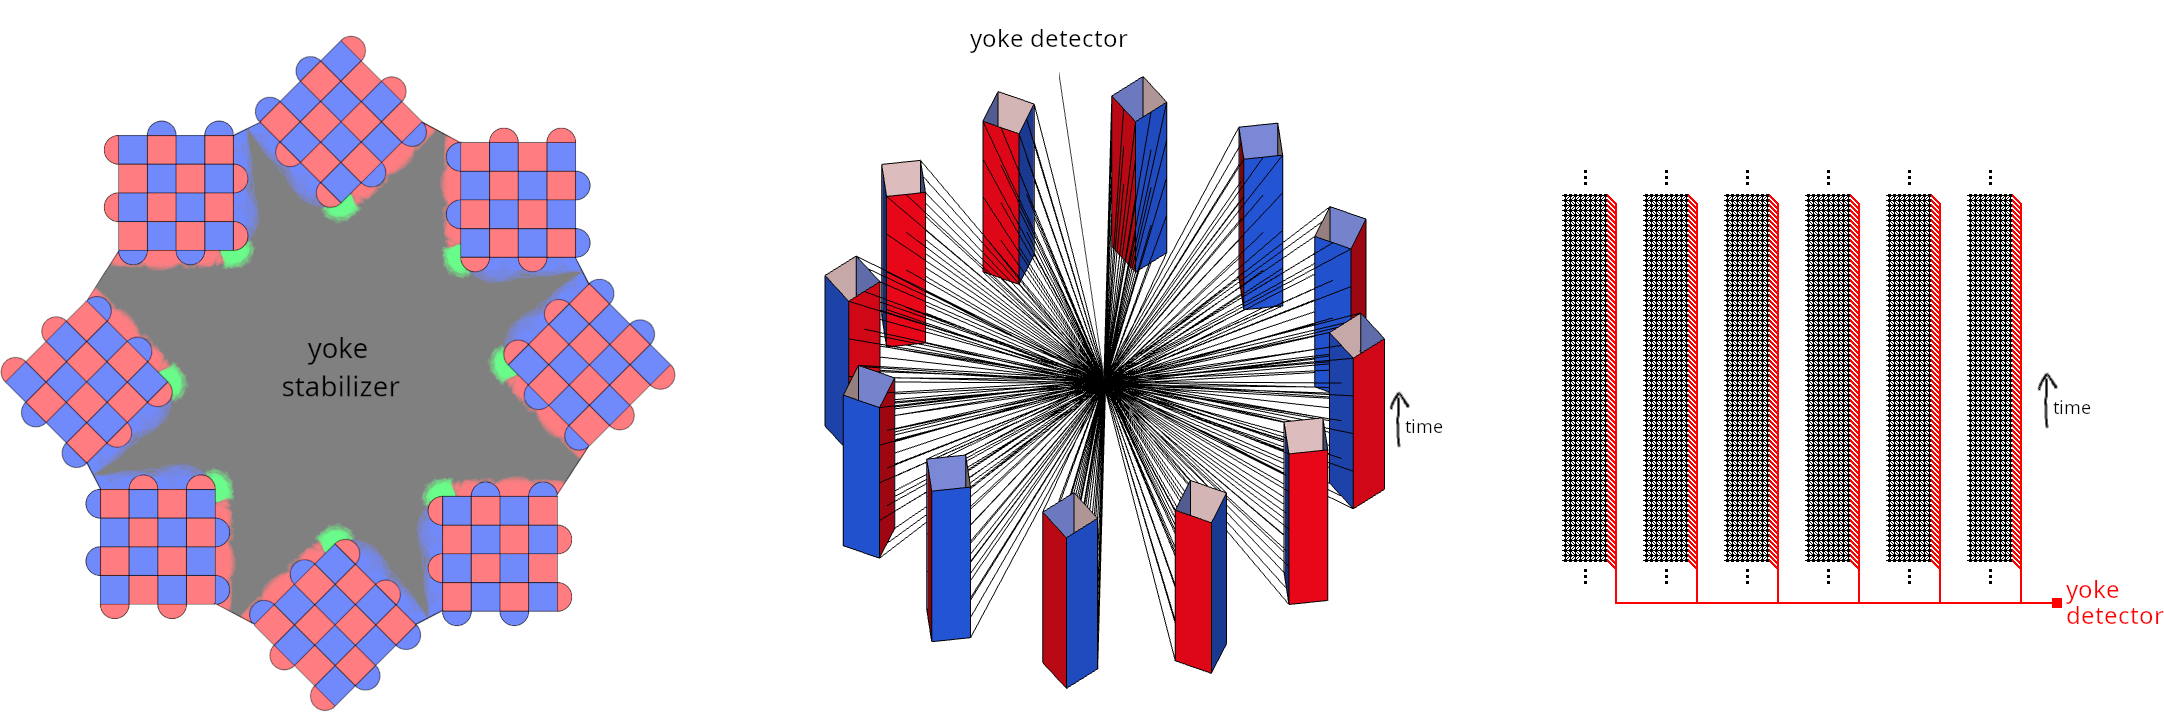
\includegraphics{assets/yoke_diagram.png}
    }
    \caption{
        Various depictions of yoked codes.
        Left: a stabilizer configuration diagram of eight surface codes yoked by a central $Y_L^{\otimes 8}$ stabilizer.
        Middle: a mix of a defect diagram and a match graph diagram, showing twelve idle surface codes yoked by a $Y_L^{\otimes 12}$ stabilizer.
        The central node linked to by all the boundaries is the detector node corresponding to comparing the yoke's value before and after the shown time range.
        Right: match graph diagram of six repetition codes yoked by a $Z_L^{\otimes 6}$ stabilizer.
        All edges in the match graph that would have been a right-side boundary edge are instead an edge to the yoke detector node.
    }
    \label{fig:yoke_depictions}
\end{figure}




\section{Construction}
\label{sec:construction}

\subsection{Anti-Y Bias in Surface Codes}

The surface code doesn't treat the Pauli bases symmetrically.
At the microscopic level, modulo single qubit rotations, the surface code is built out of X stabilizers and Z stabilizers.
It has no Y stabilizers.
At the macroscopic level, a surface code computation is defined by the arrangement of topological defects.
The X and Z defects (``boundaries'') form 2D surfaces in spacetime, while the Y type defects (``twists'') form 1D curves~\cite{brown2017surfacetwists,gidneyinplaceybasis2023}.

A consequence of these asymmetries is that, when a surface code fails, the failure is unlikely to be a logical Y error.
It's more likely for errors to travel from side to opposite side (producing an X type or Z type error), rather than from corner to opposite corner (producing a Y type error).
In \sec{benchmarking} we perform simulations quantifying this bias.

Some readers may be aware that, under phenomenological noise, a rotated surface code patch of diameter $d$ has no distance $d$ error mechanism that produces a logical Y error.
Under circuit noise, this changes.
Halfway through the cycle circuit, there are two qubit gates aligned diagonally, creating a highway between diagonally opposite corners.
Two qubit depolarization on $d$ of these gates can be used to cause a logical $Y$ error while producing no detection events, and so the Y code distance is $d$.
However, although strictly speaking the Y distance is $d$ under circuit noise, the logical Y error mechanisms are so specific and esoteric compared to the logical X and Z error mechanisms that it's misleading to describe them using the same number.
In simulation, we see that a better approximation is to pretend that a distance $d$ surface code patch has a Y code distance of $1.8d$.


\subsection{Iceberg codes and Yberg codes}

An iceberg code~\cite{steane1996simpleqec,self2022iceberg} is an $[[n, n-2, 2]]$ code built out of one $X^{\otimes n}$ stabilizer and one $Z^{\otimes n}$ stabilizer (see \tab{codes}; $n$ must be even).
Iceberg codes have a code distance of 2, and a nearly perfect coding rate of $n-2:n$.
It's impossible to achieve a better coding rate, while maintaining the property that any individual single qubit error can be detected.

Motivated by the surface code's bias away from Y errors, we define a variant of iceberg codes with just one $Y^{\otimes n}$ stabilizer.
We call this code family ``Yberg codes'' (see \tab{codes}).
Yberg codes can't detect Y errors, so they have a code distance of 1.
However, for the purposes of this paper, we'll refer to them as having a code distance of ``1.8'' because, in our simulations, distance $d$ surface codes had a $Y$ error rate roughly equal to the X or Z error rate of a distance $1.8d$ surface code.

\begin{table}[h]
    \centering
    \begin{tabular}{|c|c|c|}
        \hline
        \multicolumn{3}{|c|}{[[10, 8, 2]] Iceberg Code} \\
        \hline
        Check & Stabilizer & - \\
        \hline
        1 & \texttt{XXXXXXXXXX} & - \\
        2 & \texttt{ZZZZZZZZZZ} & - \\
        \hline
        Qubit & X Observable & Z Observable \\
        \hline
        1 & \texttt{X\_\_\_\_\_\_\_X\_} & \texttt{Z\_\_\_\_\_\_\_\_Z} \\
        2 & \texttt{\_X\_\_\_\_\_\_X\_} & \texttt{\_Z\_\_\_\_\_\_\_Z} \\
        3 & \texttt{\_\_X\_\_\_\_\_X\_} & \texttt{\_\_Z\_\_\_\_\_\_Z} \\
        4 & \texttt{\_\_\_X\_\_\_\_X\_} & \texttt{\_\_\_Z\_\_\_\_\_Z} \\
        5 & \texttt{\_\_\_\_X\_\_\_X\_} & \texttt{\_\_\_\_Z\_\_\_\_Z} \\
        6 & \texttt{\_\_\_\_\_X\_\_X\_} & \texttt{\_\_\_\_\_Z\_\_\_Z} \\
        7 & \texttt{\_\_\_\_\_\_X\_X\_} & \texttt{\_\_\_\_\_\_Z\_\_Z} \\
        8 & \texttt{\_\_\_\_\_\_\_XX\_} & \texttt{\_\_\_\_\_\_\_Z\_Z} \\
        \hline
    \end{tabular}
    \hfill
    \begin{tabular}{|c|c|c|}
        \hline
        \multicolumn{3}{|c|}{[[9, 8, 1.8]] Yberg Code} \\
        \hline
        Check & Stabilizer & - \\
        \hline
        1 & \texttt{YYYYYYYYY} & - \\
        \hline
        Qubit & X Observable & Z Observable \\
        \hline
        1 & \texttt{X\_\_\_\_\_\_\_X} & \texttt{Z\_\_\_\_\_\_\_X} \\
        2 & \texttt{\_X\_\_\_\_\_\_X} & \texttt{\_Z\_\_\_\_\_\_X} \\
        3 & \texttt{\_\_X\_\_\_\_\_X} & \texttt{\_\_Z\_\_\_\_\_X} \\
        4 & \texttt{\_\_\_X\_\_\_\_X} & \texttt{\_\_\_Z\_\_\_\_X} \\
        5 & \texttt{\_\_\_\_X\_\_\_X} & \texttt{\_\_\_\_Z\_\_\_X} \\
        6 & \texttt{\_\_\_\_\_X\_\_X} & \texttt{\_\_\_\_\_Z\_\_X} \\
        7 & \texttt{\_\_\_\_\_\_X\_X} & \texttt{\_\_\_\_\_\_Z\_X} \\
        8 & \texttt{\_\_\_\_\_\_\_XX} & \texttt{\_\_\_\_\_\_\_ZX} \\
        \hline
    \end{tabular}
    \caption{
        Definitions of stabilizers and observables in the $n=10,k=8,d=2$ iceberg code and the $n=9,k=8,d=1.8$ Yberg code.
        The Yberg code's distance is listed as ``1.8'' because \fig{bias} indicates a distance $d$ surface code has a Y error rate roughly equal to the X or Z error rate of a distance $1.8d$ surface code.
    }
    \label{tab:codes}
\end{table}


\subsection{Complementary Gaps}

The surface code can be decoded by minimum weight perfect matching.
The edges of the minimum weight matching identify a correction to perform.
Instead of only returning this one matching, the decoder can be modified to also return a second minimum weight matching where the second matching is constrained to give a topologically distinct logical correction~\cite{hutter2014complementarygap,bombin2022postselect}.
This is the ``complementary matching''.
The difference in weight between the normal matching and the complementary matching is ``the complementary gap'' or just ``the gap'' for short.

In a surface code memory experiment, there is a surprisingly simple way to compute a complementary matching~\cite{hutter2014complementarygap,bombin2022postselect}: pretend a boundary is actually a detector, excite this detector, and see how the decoder gets rid of the excitation.
The only way to get rid of this extra excitation is to push it across the patch, to the boundary on the opposite side, forcing the decoder into a topologically distinct solution.
Decoding the case with the boundary-detector excited, and also the case with it not excited, will produce two matchings.
One of the matchings will have the lower weight, and corresponds to the usual minimum weight matching.
The higher weight solution is the complementary matching.
The absolute difference in their weights is the gap.

In \sec{benchmarking} we'll show that the gap is a well calibrated predictor of whether a logical error has occurred.
We'll also show sampled distributions of gaps, and how to extrapolate these distributions to large numbers of rounds.


\subsection{Yoking and Boundary Hugging}

Our construction is to concatenate an iceberg code, or Yberg code, over the surface code and to use the complementary gap as tie breaking soft information.
When an error is detected by a yoke, we correct it by flipping the lowest-gap observable out of the observables protected by that yoke.
To explain yoking to existing decoders, we use a trick we call ``boundary hugging''.
Boundary hugging was also used in \cite{lessbaconmorethreshold2023}, to explain concatenated Bacon-Shor codes to existing decoders.

In the surface code, the X and Z logical observables correspond to a path from one boundary to the boundary on the opposite side of the patch.
We can pick which specific path we declare as the observable.
For example, an observable going from the bottom of a patch to the top of the patch could run through the middle, or along the left side, or along the right side, or many other options.
Yokes are products of patch observables, and so the same freedom of path choice applies.
When we explain a yoke to a decoder, we can choose to explain it in a way that puts the yoke next to boundaries.
For observables this choice wouldn't matter; it just affects the labelling of edges given to the decoder.
But when it comes to explaining yokes to existing decoders, this is a key detail.

In order for the yoke to be understood by the decoder, the yoke needs to be presented as a node in the matching graph (i.e. as a detector).
If we run the yoke along the middle of a patch, the physical errors that flip the yoke will be errors along the middle of the patch.
This means those errors will have three symptoms: the usual two bulk detection events, plus a detection event on the yoke detector.
This is a major problem because the error is now effectively a hyper edge in the matching graph, instead of a normal edge.
Matching-based decoders don't understand hyper edges.
If we instead run the yoke along the boundary of the patch then, instead of turning normal edges into hyper edges, the yoke will turn boundary edges into normal edges.
Matching-based decoders understand normal edges, and therefore they understand this boundary hugging yoke.
If we want existing decoders to understand our yokes then we need to maintain this boundary hugging property, including during complex operations such as lattice surgery.

Although we think presenting a yoke to the decoder as a normal detector node is a good hack, it has several important limitations.
First, when using boundary hugging, a detector node corresponding to a yoke will have thousands of neighbors reaching far across the matching graph.
This can cause performance problems in the decoder, and it makes it difficult to cut the decoding problem into pieces.
Second, maintaining boundary hugging introduces restrictions on how logical operations are performed.
For example, we may need to rotate a patch clockwise instead of counter-clockwise (whereas normally this wouldn't matter) or we may not be able to perform lattice surgery at the earliest possible time.
We believe these restrictions and performance problems are all solvable, but they require changing the decoder.
We leave this as future work.


\subsection{Measuring Yokes with Lattice Surgery}

A key detail, when concatenating a code over the surface code, is how the stabilizers of the overlying code will be measured.
It's not reasonable to ignore this detail, because the workspace needed to periodically measure the stabilizers of the overlying code can easily be larger than the space needed to just store the qubits.
Also, the effects of errors occurring during the lattice surgery need to be accounted for in order to understand the behavior of the overlying code.

Originally, lattice surgery was thought of as being built out of parity measurements~\cite{horsman2012latticesurgery,fowler2018latticesurgery}.
But a far more useful perspective is to view lattice surgery as an instantiation of the ZX calculus~\cite{de2017zxlattice}.
In the latter perspective, the building blocks of lattice surgery are not operations on qubits but rather connections between junctions.
Making a good lattice surgery construction then becomes an exercise in packing and routing and rotating pipes, so that they link together in the required way.

In \fig{iceberg_check} and \fig{yberg_check} we present ZX graphs implementing the stabilizer checks for iceberg codes and Yberg codes, alongside the corresponding lattice surgery implementations.
These constructions satisfy the boundary hugging constraint, except for the odd $n$ Yberg construction (meaning we'll avoid using odd $n$ Yberg codes in our final estimates).
All locations in the iceberg lattice surgery construction are protected by one of the four yokes present (the ending $X^{\otimes n}$, the ending $Z^{\otimes n}$, the starting $X^{\otimes n}$, or the starting $Z^{\otimes n}$).
The Yberg code construction has one location that is only partially protected: some X and Z errors next to the yellow Hadamard box are undetected.
This is a small enough portion of the construction that it can likely be ignored, because it's acceptable to have higher logical error rates in rare places.
The cautious reader may wish to stretch out the partially protected parts of the construction, increasing the code distance against any errors that wouldn't be detected by a yoke.

These constructions use the patch rotation from \cite{litinski2019gameofsurfacecodes}, shown in \fig{patch_rotation}.
One worry we had was that this rotation may have different noise characteristics than idling (e.g. less Y bias).
In \sec{benchmarking} we show that the patch rotation has errors essentially identical to idling (see \fig{bias}).

Based on the above analysis of the error mechanisms and the noise bias, we think the error cost of the lattice surgery should be reasonably well represented by the error cost of idling.
So, in \sec{benchmarking}, we will focus on simulations of idling when attempting to understand how error rates behave.


\begin{figure}[h]
    \centering
    \resizebox{\linewidth}{!}{
        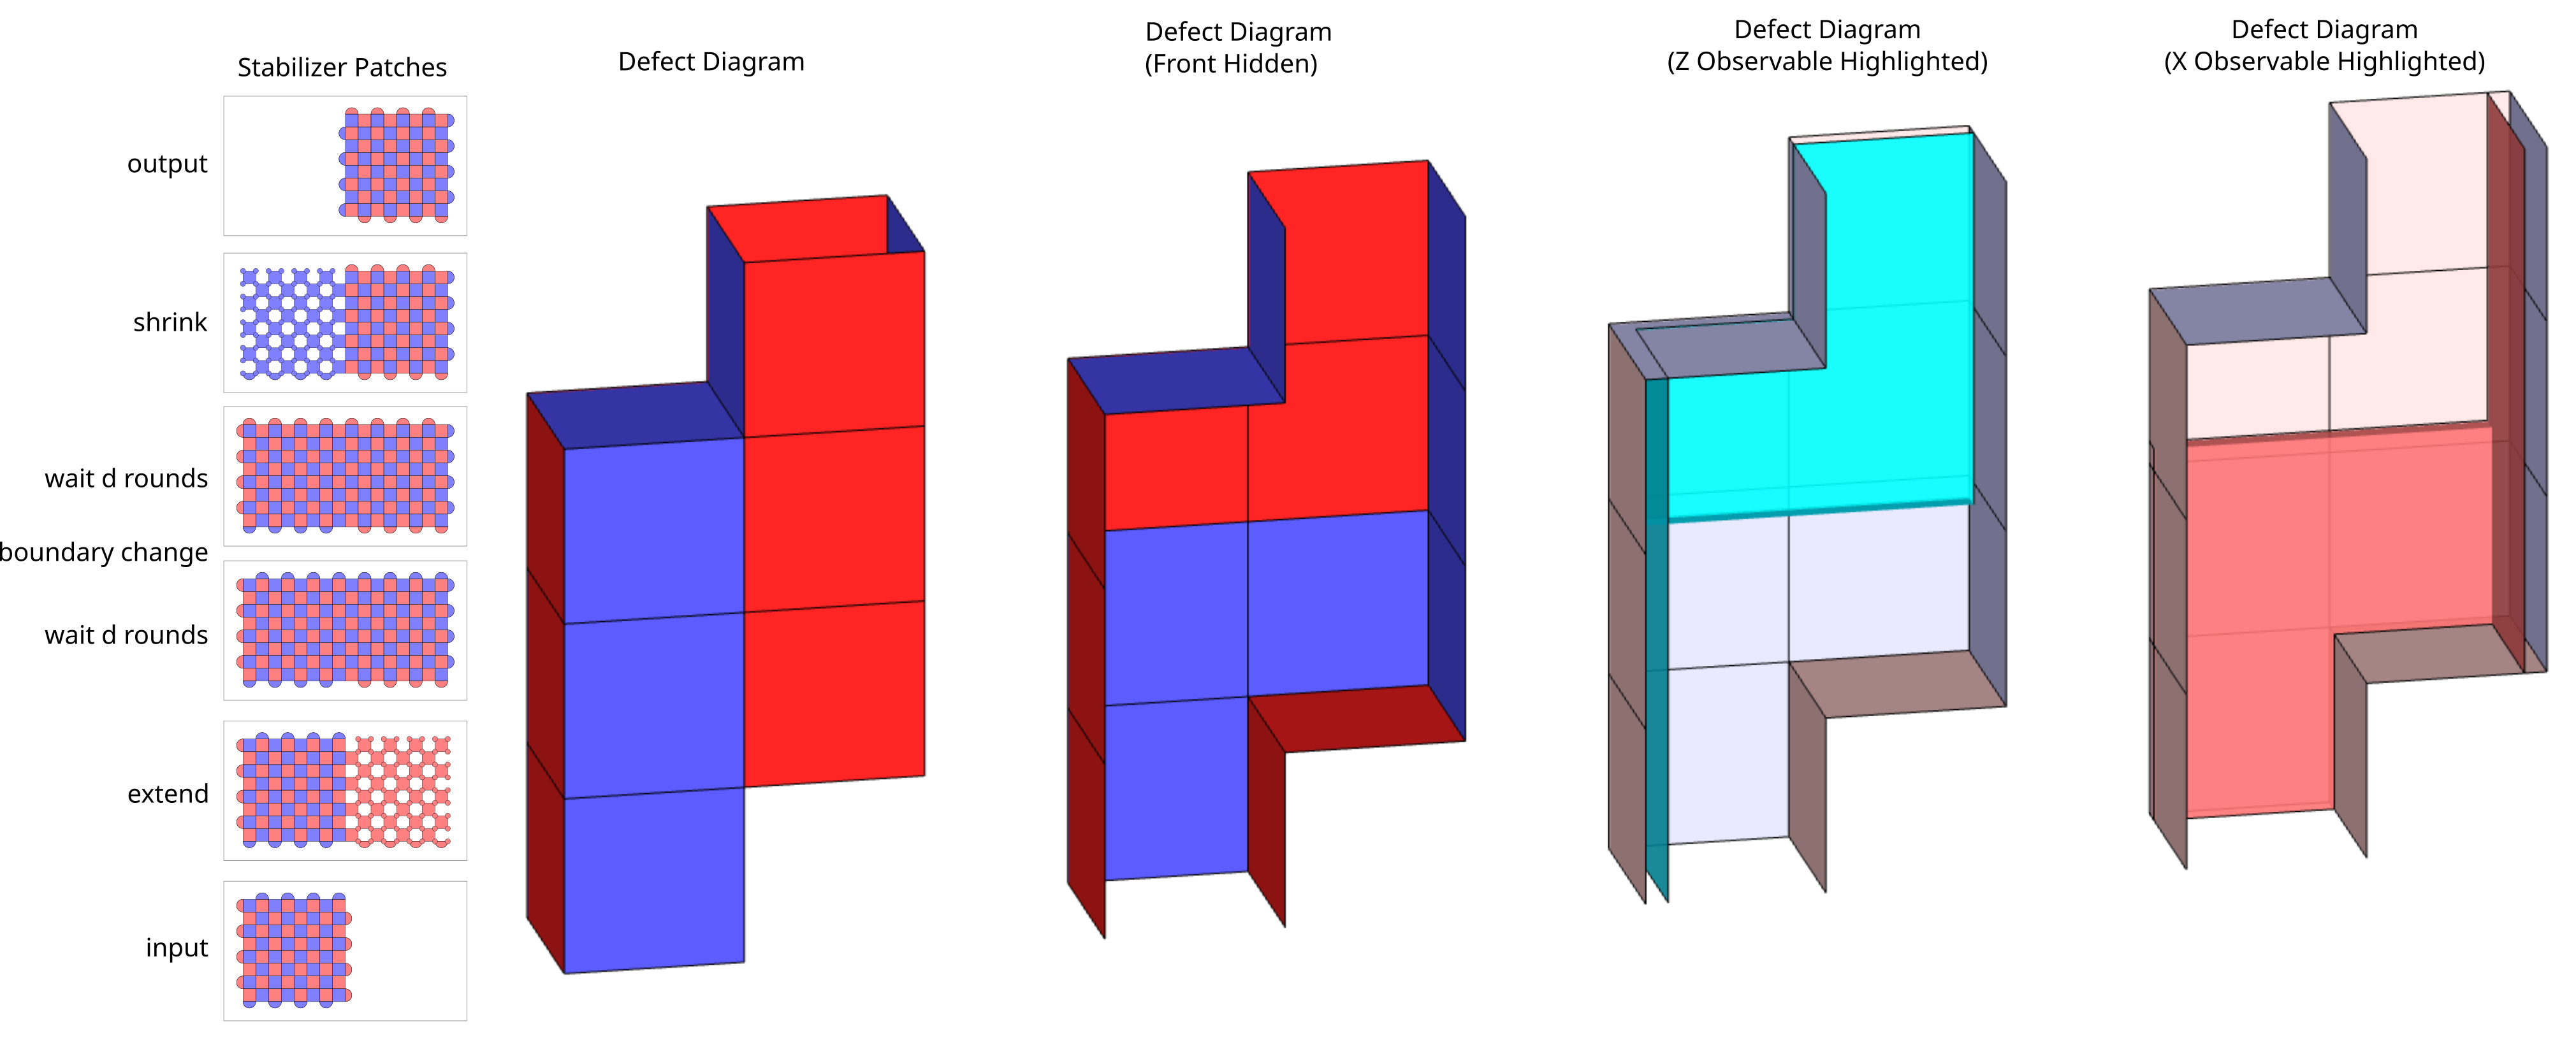
\includegraphics{assets/patch_rotation.png}
    }
    \caption{
        The patch rotation construction from \cite{litinski2019gameofsurfacecodes}, with the last step omitted, leaving the patch shifted as part of the rotation.
    }
    \label{fig:patch_rotation}
\end{figure}

\begin{figure}[h]
    \centering
    \resizebox{\linewidth}{!}{
        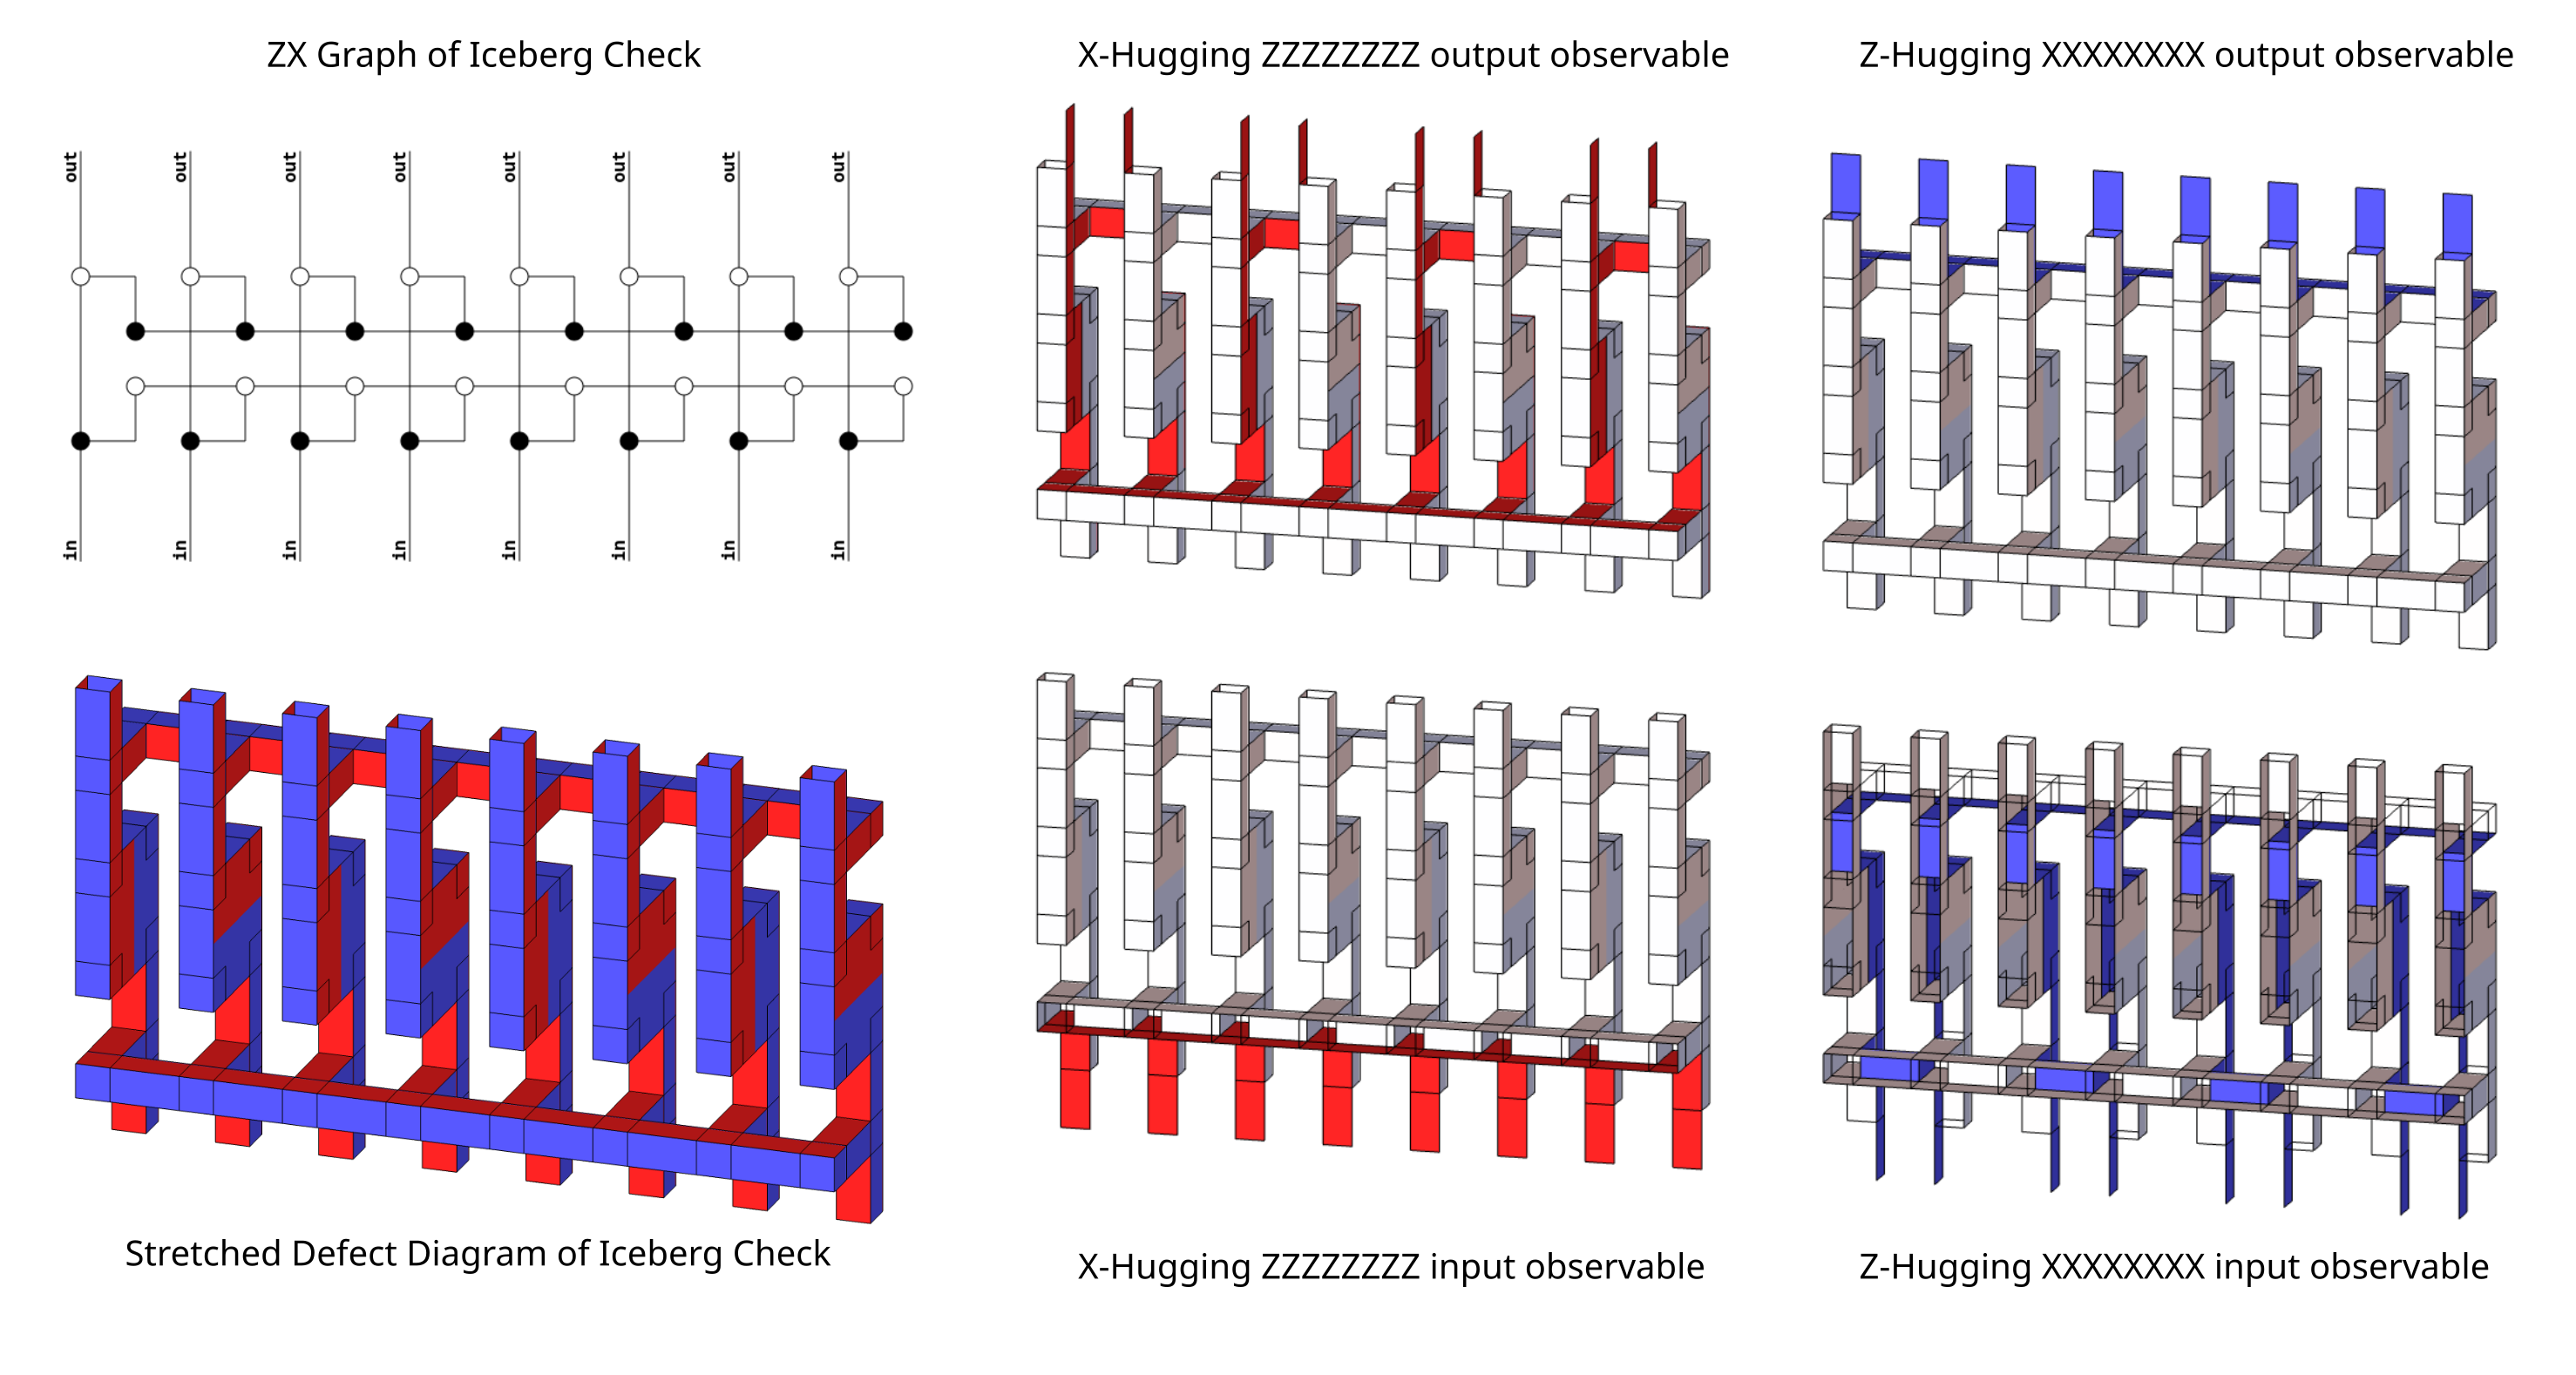
\includegraphics{assets/iceberg_check.png}
    }
    \caption{
        How to check the $X^{\otimes n}$ and $Z^{\otimes n}$ stabilizers of the iceberg code using lattice surgery.
        The stabilizer flows of \href{https://algassert.com/zigxag\#1,2,out;3,2,out;5,2,out;7,2,out;9,2,out;11,2,out;13,2,out;15,2,out;1,3,+;3,3,+;5,3,+;7,3,+;9,3,+;11,3,+;13,3,+;15,3,+;1,4,O;2,4,+;3,4,O;4,4,+;5,4,O;6,4,+;7,4,O;8,4,+;9,4,O;10,4,+;11,4,O;12,4,+;13,4,O;14,4,+;15,4,O;16,4,+;1,5,+;2,5,@;3,5,+;4,5,@;5,5,+;6,5,@;7,5,+;8,5,@;9,5,+;10,5,@;11,5,+;12,5,@;13,5,+;14,5,@;15,5,+;16,5,@;1,6,+;2,6,O;3,6,+;4,6,O;5,6,+;6,6,O;7,6,+;8,6,O;9,6,+;10,6,O;11,6,+;12,6,O;13,6,+;14,6,O;15,6,+;16,6,O;1,7,@;2,7,+;3,7,@;4,7,+;5,7,@;6,7,+;7,7,@;8,7,+;9,7,@;10,7,+;11,7,@;12,7,+;13,7,@;14,7,+;15,7,@;16,7,+;1,8,+;3,8,+;5,8,+;7,8,+;9,8,+;11,8,+;13,8,+;15,8,+;1,9,in;3,9,in;5,9,in;7,9,in;9,9,in;11,9,in;13,9,in;15,9,in:1,2,1,3,-;3,2,3,3,-;5,2,5,3,-;7,2,7,3,-;9,2,9,3,-;11,2,11,3,-;13,2,13,3,-;15,2,15,3,-;1,3,1,4,-;3,3,3,4,-;5,3,5,4,-;7,3,7,4,-;9,3,9,4,-;11,3,11,4,-;13,3,13,4,-;15,3,15,4,-;1,4,2,4,-;1,4,1,5,-;2,4,2,5,-;3,4,4,4,-;3,4,3,5,-;4,4,4,5,-;5,4,6,4,-;5,4,5,5,-;6,4,6,5,-;7,4,8,4,-;7,4,7,5,-;8,4,8,5,-;9,4,10,4,-;9,4,9,5,-;10,4,10,5,-;11,4,12,4,-;11,4,11,5,-;12,4,12,5,-;13,4,14,4,-;13,4,13,5,-;14,4,14,5,-;15,4,16,4,-;15,4,15,5,-;16,4,16,5,-;1,5,1,6,-;2,5,3,5,-;3,5,4,5,-;3,5,3,6,-;4,5,5,5,-;5,5,6,5,-;5,5,5,6,-;6,5,7,5,-;7,5,8,5,-;7,5,7,6,-;8,5,9,5,-;9,5,10,5,-;9,5,9,6,-;10,5,11,5,-;11,5,12,5,-;11,5,11,6,-;12,5,13,5,-;13,5,14,5,-;13,5,13,6,-;14,5,15,5,-;15,5,16,5,-;15,5,15,6,-;1,6,1,7,-;2,6,3,6,-;2,6,2,7,-;3,6,4,6,-;3,6,3,7,-;4,6,5,6,-;4,6,4,7,-;5,6,6,6,-;5,6,5,7,-;6,6,7,6,-;6,6,6,7,-;7,6,8,6,-;7,6,7,7,-;8,6,9,6,-;8,6,8,7,-;9,6,10,6,-;9,6,9,7,-;10,6,11,6,-;10,6,10,7,-;11,6,12,6,-;11,6,11,7,-;12,6,13,6,-;12,6,12,7,-;13,6,14,6,-;13,6,13,7,-;14,6,15,6,-;14,6,14,7,-;15,6,16,6,-;15,6,15,7,-;16,6,16,7,-;1,7,2,7,-;1,7,1,8,-;3,7,4,7,-;3,7,3,8,-;5,7,6,7,-;5,7,5,8,-;7,7,8,7,-;7,7,7,8,-;9,7,10,7,-;9,7,9,8,-;11,7,12,7,-;11,7,11,8,-;13,7,14,7,-;13,7,13,8,-;15,7,16,7,-;15,7,15,8,-;1,8,1,9,-;3,8,3,9,-;5,8,5,9,-;7,8,7,9,-;9,8,9,9,-;11,8,11,9,-;13,8,13,9,-;15,8,15,9,-}{the ZX calculus graph} can be evaluated to confirm the $X^{\otimes n}$ and $Z^{\otimes n}$ stabilizers are being measured, and that the encoded logical qubits are being propagated.
        The defect diagrams aren't to scale; the connections between pieces are stretched out to show the topology.
        The process occupies $2 \times n$ logical qubit patches for $4d$ rounds.
        The patch rotations are alternating between left handed and right handed, to satisfy the boundary hugging constraint.
        The defect diagrams with highlighted observables show how the yoke stabilizers are measured and prepared.
    }
    \label{fig:iceberg_check}
\end{figure}

\begin{figure}[h]
    \centering
    \resizebox{\linewidth}{!}{
        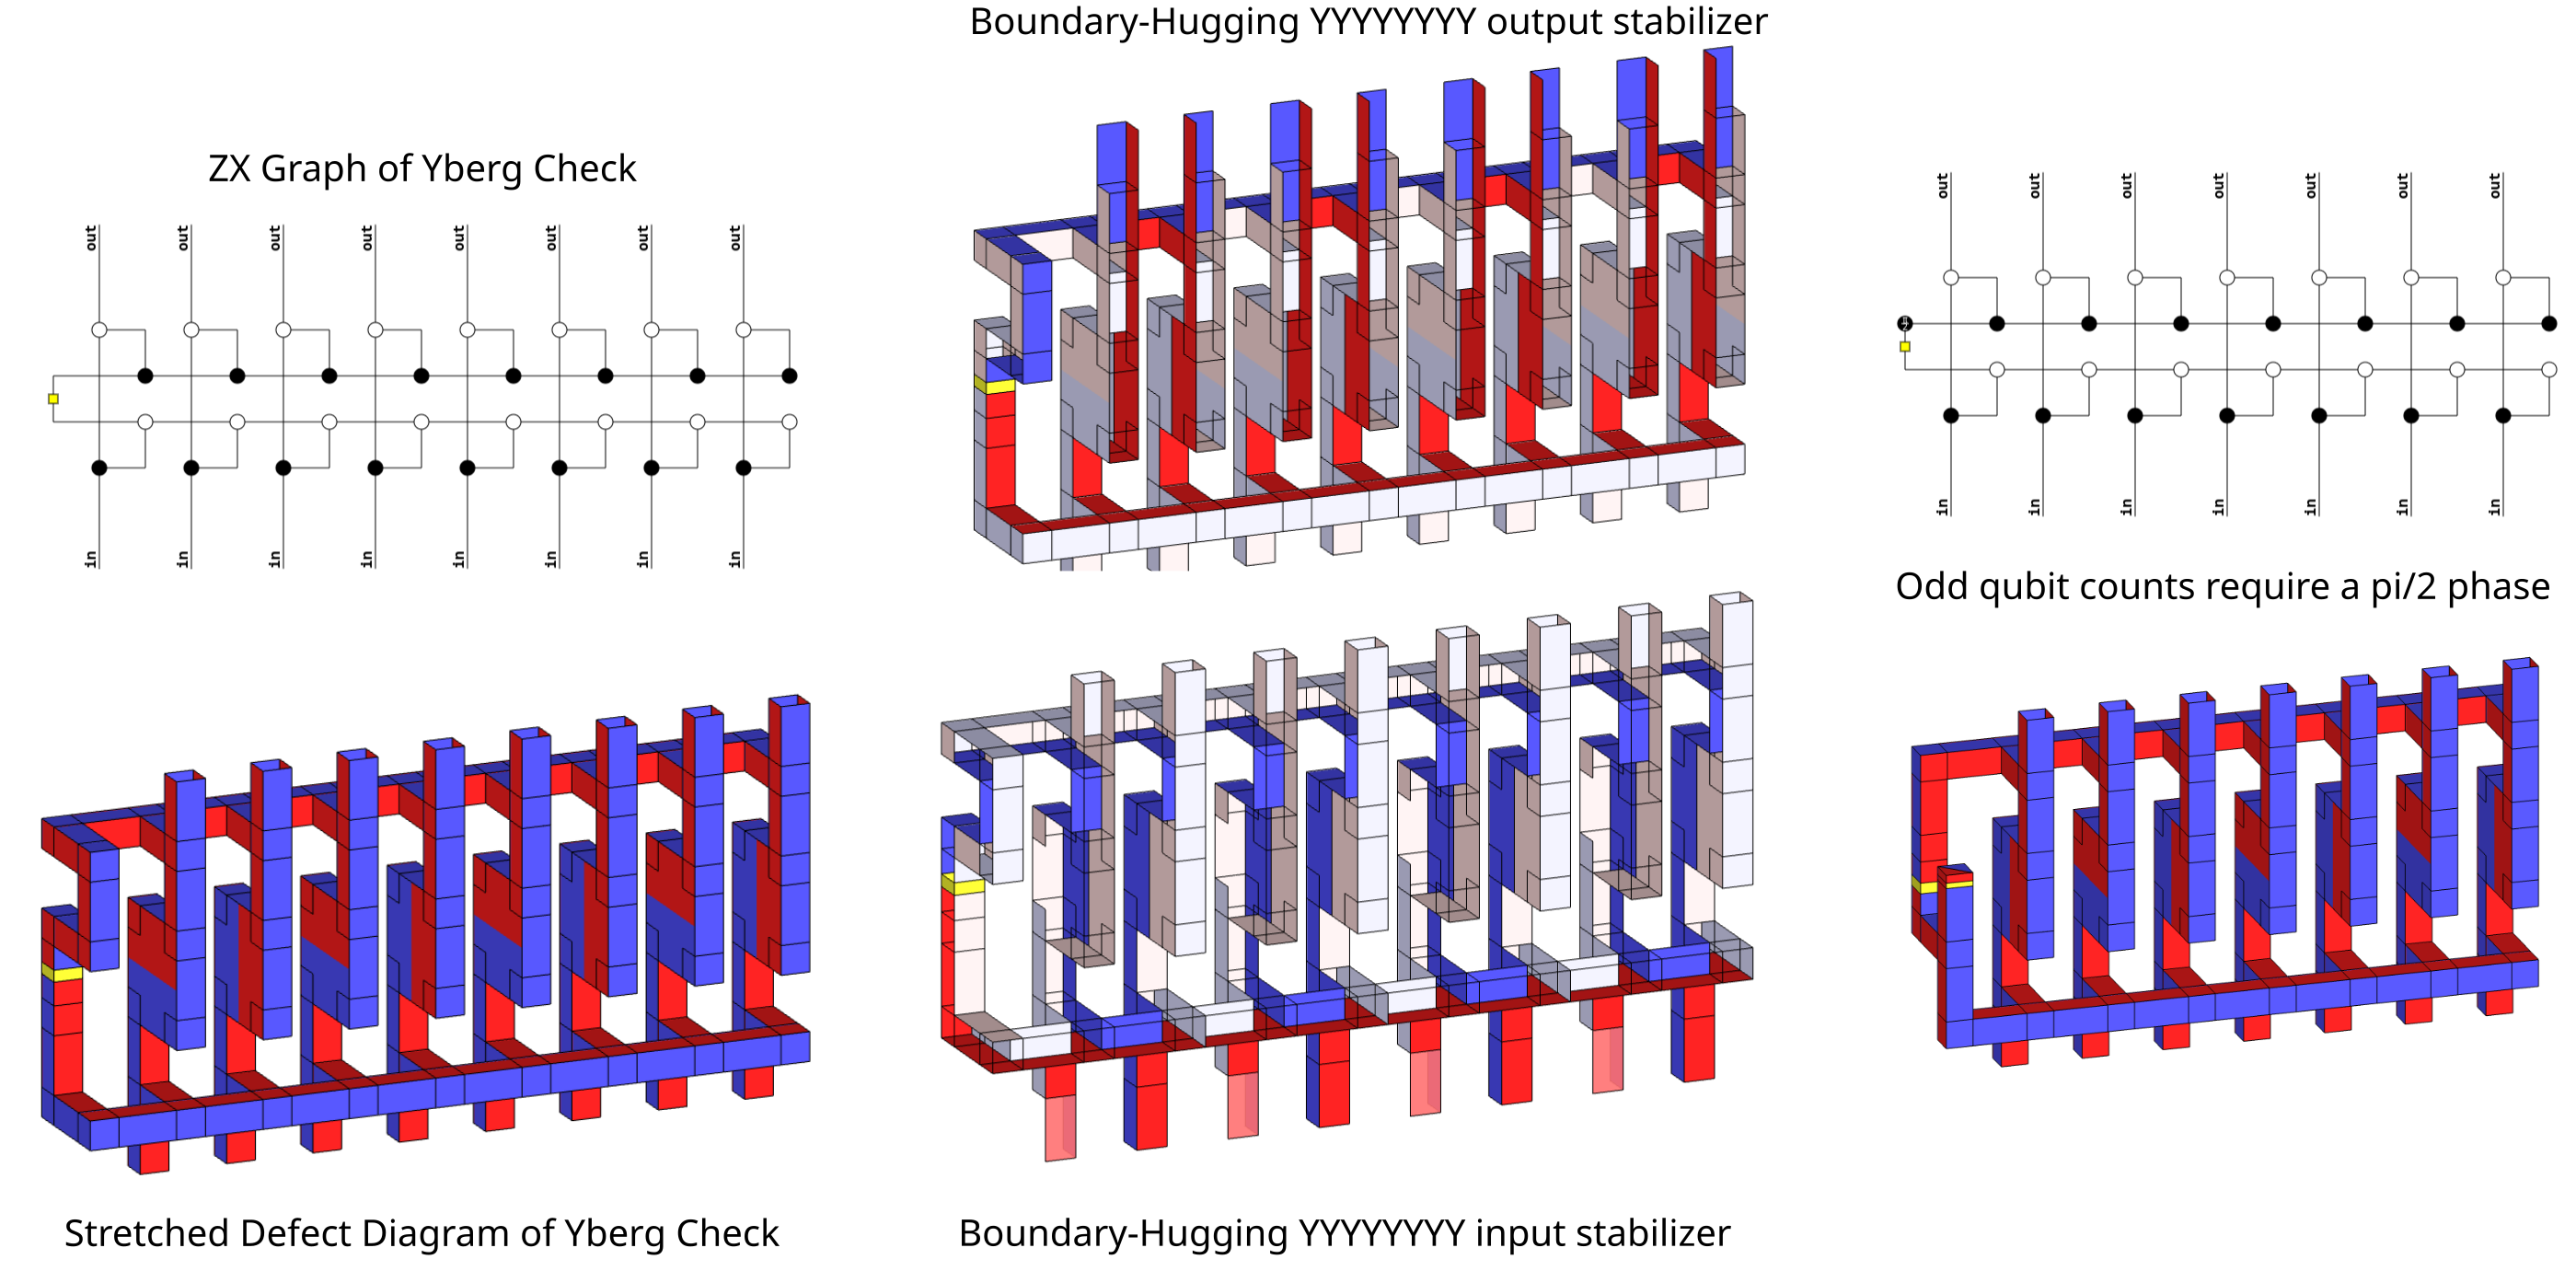
\includegraphics{assets/yberg_check.png}
    }
    \caption{
        How to check the $Y^{\otimes n}$ stabilizer of the Yberg code using lattice surgery.
        The stabilizer flows of \href{https://algassert.com/zigxag\#1,2,out;3,2,out;5,2,out;7,2,out;9,2,out;11,2,out;13,2,out;15,2,out;1,3,+;3,3,+;5,3,+;7,3,+;9,3,+;11,3,+;13,3,+;15,3,+;1,4,O;2,4,+;3,4,O;4,4,+;5,4,O;6,4,+;7,4,O;8,4,+;9,4,O;10,4,+;11,4,O;12,4,+;13,4,O;14,4,+;15,4,O;16,4,+;0,5,+;1,5,+;2,5,@;3,5,+;4,5,@;5,5,+;6,5,@;7,5,+;8,5,@;9,5,+;10,5,@;11,5,+;12,5,@;13,5,+;14,5,@;15,5,+;16,5,@;0,6,+;1,6,+;2,6,O;3,6,+;4,6,O;5,6,+;6,6,O;7,6,+;8,6,O;9,6,+;10,6,O;11,6,+;12,6,O;13,6,+;14,6,O;15,6,+;16,6,O;1,7,@;2,7,+;3,7,@;4,7,+;5,7,@;6,7,+;7,7,@;8,7,+;9,7,@;10,7,+;11,7,@;12,7,+;13,7,@;14,7,+;15,7,@;16,7,+;1,8,+;3,8,+;5,8,+;7,8,+;9,8,+;11,8,+;13,8,+;15,8,+;1,9,in;3,9,in;5,9,in;7,9,in;9,9,in;11,9,in;13,9,in;15,9,in:1,2,1,3,-;3,2,3,3,-;5,2,5,3,-;7,2,7,3,-;9,2,9,3,-;11,2,11,3,-;13,2,13,3,-;15,2,15,3,-;1,3,1,4,-;3,3,3,4,-;5,3,5,4,-;7,3,7,4,-;9,3,9,4,-;11,3,11,4,-;13,3,13,4,-;15,3,15,4,-;1,4,2,4,-;1,4,1,5,-;2,4,2,5,-;3,4,4,4,-;3,4,3,5,-;4,4,4,5,-;5,4,6,4,-;5,4,5,5,-;6,4,6,5,-;7,4,8,4,-;7,4,7,5,-;8,4,8,5,-;9,4,10,4,-;9,4,9,5,-;10,4,10,5,-;11,4,12,4,-;11,4,11,5,-;12,4,12,5,-;13,4,14,4,-;13,4,13,5,-;14,4,14,5,-;15,4,16,4,-;15,4,15,5,-;16,4,16,5,-;0,5,1,5,-;0,5,0,6,h;1,5,2,5,-;1,5,1,6,-;2,5,3,5,-;3,5,4,5,-;3,5,3,6,-;4,5,5,5,-;5,5,6,5,-;5,5,5,6,-;6,5,7,5,-;7,5,8,5,-;7,5,7,6,-;8,5,9,5,-;9,5,10,5,-;9,5,9,6,-;10,5,11,5,-;11,5,12,5,-;11,5,11,6,-;12,5,13,5,-;13,5,14,5,-;13,5,13,6,-;14,5,15,5,-;15,5,16,5,-;15,5,15,6,-;0,6,1,6,-;1,6,2,6,-;1,6,1,7,-;2,6,3,6,-;2,6,2,7,-;3,6,4,6,-;3,6,3,7,-;4,6,5,6,-;4,6,4,7,-;5,6,6,6,-;5,6,5,7,-;6,6,7,6,-;6,6,6,7,-;7,6,8,6,-;7,6,7,7,-;8,6,9,6,-;8,6,8,7,-;9,6,10,6,-;9,6,9,7,-;10,6,11,6,-;10,6,10,7,-;11,6,12,6,-;11,6,11,7,-;12,6,13,6,-;12,6,12,7,-;13,6,14,6,-;13,6,13,7,-;14,6,15,6,-;14,6,14,7,-;15,6,16,6,-;15,6,15,7,-;16,6,16,7,-;1,7,2,7,-;1,7,1,8,-;3,7,4,7,-;3,7,3,8,-;5,7,6,7,-;5,7,5,8,-;7,7,8,7,-;7,7,7,8,-;9,7,10,7,-;9,7,9,8,-;11,7,12,7,-;11,7,11,8,-;13,7,14,7,-;13,7,13,8,-;15,7,16,7,-;15,7,15,8,-;1,8,1,9,-;3,8,3,9,-;5,8,5,9,-;7,8,7,9,-;9,8,9,9,-;11,8,11,9,-;13,8,13,9,-;15,8,15,9,-}{the ZX calculus graph} can be evaluated to confirm the $Y^{\otimes n}$ stabilizer is being measured, and that the encoded logical qubits are being propagated.
        The defect diagrams aren't to scale; the connections between pieces are stretched out to show the topology.
        The process occupies $2 \times n$ logical qubit patches for $4d$ rounds.
        The patch rotations are alternating between left handed and right handed, to satisfy the boundary hugging constraint.
        The defect diagrams with highlighted observables show how the yoke stabilizer is measured and prepared.
        The yellow ring indicates a timelike domain wall, implemented using the walking surface code~\cite{mcewen2022relaxing} and a transversal layer of Hadamards.
        Note that the shown odd qubit count construction doesn't satisfy the boundary hugging constraint, so we avoid using it in this paper.
    }
    \label{fig:yberg_check}
\end{figure}


\subsection{Hot and Cold Storage Architectures}

Above the abstraction level of lattice surgery is the notion of a storage architecture.
In this paper we consider two different storage architectures, which we call ``cold storage'' and ``hot storage''.

In ``cold storage'', qubits are stored in a form where they are as dense as possible but can't be immediately operated upon.
Operating on a qubit in cold storage requires first getting it out of storage.
Concretely, this means the qubits don't all have access hallways next to them.
It's still necessary for some workspace to be present, because it's necessary to periodically check the yokes, but this workspace can be shared between many groups of qubits.
\fig{storage} shows the space layout, and spacetime layout, that we will be using for estimates of the size of cold storage.

Qubits in ``hot storage'' are available to be operated upon.
Each qubit has a boundary exposed to an access hallway that provides a route from outside the storage to the qubit.
The existence of this access hallway is useful for yoked qubits, because it can be used as workspace for periodically measuring the yokes.
This means measuring the yokes has no marginal space cost; the space was already paid for.
Instead, it has a marginal spacetime volume cost, because although the access hallway was already there, it's blocked while the yoke is being measured.
\fig{storage} shows the space layout, and spacetime layout, that we will be using for estimates of the size of hot storage.

Storage can be ``even hotter'' than we consider here, by having each surface code patch expose two boundaries~\cite{litinski2019gameofsurfacecodes,litinskyhypercubeshor2023}.
We consider the additional space cost of exposing two boundaries to not be worth the benefit, and so don't consider layouts of that type.
Note that this means we're assuming that the yoked qubit patches are rotated on an as-needed basis, when lattice surgery needs to access the boundary that isn't exposed.
The need to do these rotations is a key consideration when laying out an algorithm.

Yoked qubits in hot storage can be operated on by lattice surgery while they're encoded.
Each encoded qubit's observable is spread over two surface code patches, but lattice surgery can stitch to two patches as easily as one.
In context the cost is actually identical, because the entrance to the access hallway is occupied regardless of how many patches are touched.
There are two main caveats on our ability to do lattice surgery on yoked qubits.
First, the lattice surgery may not always satisfy the boundary hugging constraint.
So the techniques we used to decode constructions in this paper may not work.
Second, because the yoke is only checked periodically, it's not known whether the lattice surgery was affected by a correction until the next yoke check finishes.
If the lattice surgery was part of performing a non-Clifford gate, the non-Clifford gate will be blocked from finishing until after the yoke is checked again.

Clearly, using yoked qubits has consequences on the large scale architecture of a quantum computer, beyond just the size of the storage.
These consequences are important to understand, but beyond the scope of this paper.
We leave it to future work.


\begin{figure}[h]
    \centering
    \resizebox{\linewidth}{!}{
        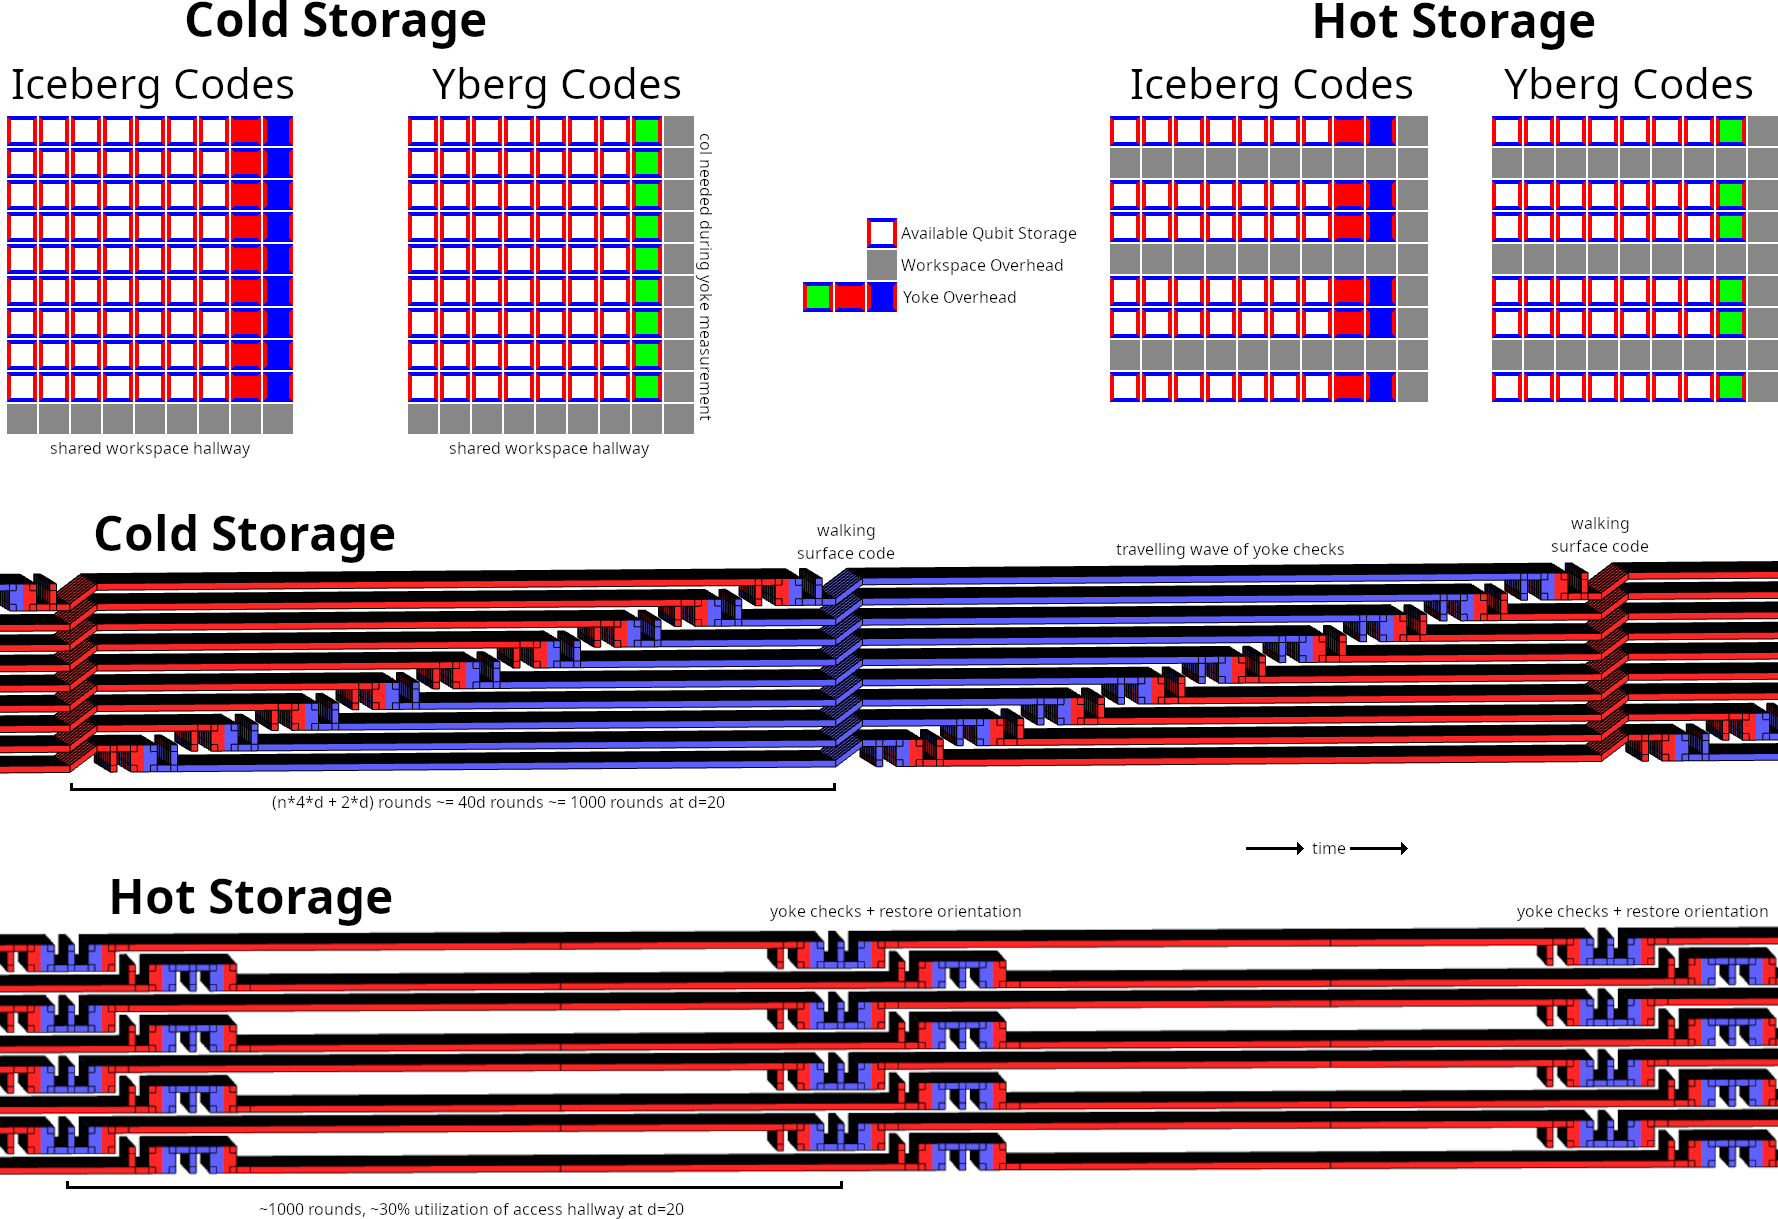
\includegraphics{assets/storage_arch.png}
    }
    \caption{
        Layouts for hot and cold storage, assuming the yoke is checked every 1000 rounds.
        The 2d footprint diagrams at the top show how space is allocated, while the 3d defect diagrams at the bottom show operations occurring over time.
        In the 2d footprint diagrams, each row is a separate group of yoked qubits.
        The white-filled squares correspond to usable storage while other squares correspond to various overheads.
        In cold storage, one row of workspace is shared between the various rows of storage in order to measure the yokes.
        In hot storage, the yokes are measured using the access hallways that would have been present anyways.
    }
    \label{fig:storage}
\end{figure}


\subsection{Scaling Laws}

Normal surface code patches have a logical error rate that scales exponentially versus patch diameter ($d$), linearly versus round count ($r$), and linearly versus patch count ($n$).
The asymptotic scaling of normal patches is $P_{\text{unyoked}} \in \Theta(r \cdot n \cdot \lambda^{-d})$ for some scaling constant $\lambda$.
A simple way to predict this scaling is to focus on the length and number of shortest error paths.
Increasing the patch diameter increases the shortest path length, which is the source of the exponential suppression versus $d$.
Doubling the number of rounds (or patches), doubles the number of shortest paths, which causes linear scaling in $r$ (and $n$).

Yoking surface code patches changes the length and number of shortest error paths.
Shortest error paths in yoked surface codes correspond to two unyoked shortest error paths meeting at the yoke (see \fig{yoke_depictions}).
Yoking doubles the code distance, but the choosing of two unyoked paths to form a yoked path introduces quadratic scaling.
Letting $r$ be more specifically the number of rounds between checks of the yoke, the number of shortest error paths in a yoked surface code scales like $\Theta(r^2 \cdot n^2)$.
Based on this, we expect the scaling of the yoked logical error rate to be $P_{\text{yoked}} \in \Theta(r \cdot r_c \cdot n^2 \cdot \lambda_2^d)$.
In \sec{benchmarking} we confirm this scaling at small sizes.

Note that the quadratic scaling versus $r$ is only for numbers of rounds up to the yoke check period.
Unyoked paths from different check periods don't combine to form a yoked error path.
So the scaling versus rounds is quadratic up to the check period, then becomes linear.

\subsection{Adaptive Yoke Checking}

In this paper, we only consider fixed yoke checking schedules.
This can almost certainly be improved upon by checking the yoke adaptively, based on conditions that arise at runtime.
For example, if a low gap event is seen, it's beneficial to check the yoke immediately; before another low gap event can occur and introduce uncertainty into the correction from the yoke.
Quantifying the amount of benefit provided by dynamic checking requires more complex simulations than we can currently perform, and a better understanding of the distribution of gaps than we currently have.
Therefore, we leave exploring this idea in detail to future work.



\section{Benchmarking}
\label{sec:benchmarking}

Simulations in this paper were performed by generating stim circuits~\cite{gidney2021stim} to describe the simulated experiments, then using sinter to orchestrate bulk sampling and decoding of these circuits by various decoders.
Pymatching is an uncorrelated minimum weight perfect matching decoder~\cite{higgott2023sparseblossom}.
In most cases we decoded shots using an internal variant of pymatching, written by Noah Shutty, that adds support for correlated matching.
In diagrams we refer to this decoder as ``sparse\_blossom\_correlated''.
In some cases we also decode shots using pymatching itself, which is labelled ``pymatching''.
Finally, in a few cases, we decode using a publication-in-progress union find decoder referred to as ``fizzle\_uncorrelated''.
These existing decoders can understand our decoding problems, despite being written without yokes in mind, because of the boundary hugging trick.

We simulated yoking with the Yberg code, yoking with the iceberg code, and not yoking at all as a control.
In diagrams: not yoking is labelled ``yokes='', yoking with Yberg codes is labelled ``yokes=1'' and yoking with iceberg codes is labelled ``yokes=2".

The circuits that we generate target the gateset $\{U_1,CZ,M_Z,R_Z\}$ and use the superconducting-inspired noise model specified in \app{noise}.
In most simulations, we use magical time boundaries where the stabilizers and observables are prepared or measured noiselessly.
The benefit of these boundaries is that they are trivial to construct, and they allow all observables to be tested simultaneously (instead of doing separate X basis and Z basis experiments).
The major downside of this approach is that the circuits can't be run on hardware.
It's also important that the circuits have many rounds, to amortize away any distortions from the perfect silence at the beginning and the end.
All circuits that we run use at least $4d$ rounds where $d$ is the patch diameter.

Most of the simulations we perform are at a noise strength of $p=0.001$.
Normally, we would simulate more varied noise strengths.
The underlying reason for focusing on one noise strength is that Monte Carlo simulation of yoked surface codes is rather expensive, because the natural size scales span orders of magnitude more qubits and rounds than normal memory experiments.
We were particularly interested in understanding scaling with respect to size, rather than with respect to noise strength, so we sacrificed noise strength diversity in favor of size diversity.

The first thing that we verified by Monte Carlo simulation was the anti-Y bias of the surface code.
We simulated $4d$-round memory experiments with various decoders, and classified each decoder mistake as $X$ or $Y$ or $Z$.
We also performed these bias simulations on a patch rotation experiment.
The patch rotation experiment also spanned $4d$ rounds, despite the fact that the patch rotation construction we used only takes $2d$ rounds, because we added $d$ rounds of idling at the beginning and the end in order to keep the patch rotation away from the magical time boundaries.
The results, shown in \fig{bias}, give two useful insights: (1) the ``effective Y distance'' of a surface code patch of diameter $d$ is roughly $1.8d$ and (2) the logical noise experienced during a patch rotation is effectively identical to the logical noise experienced while idling.

\begin{figure}[h]
    \centering
    \resizebox{\linewidth}{!}{
        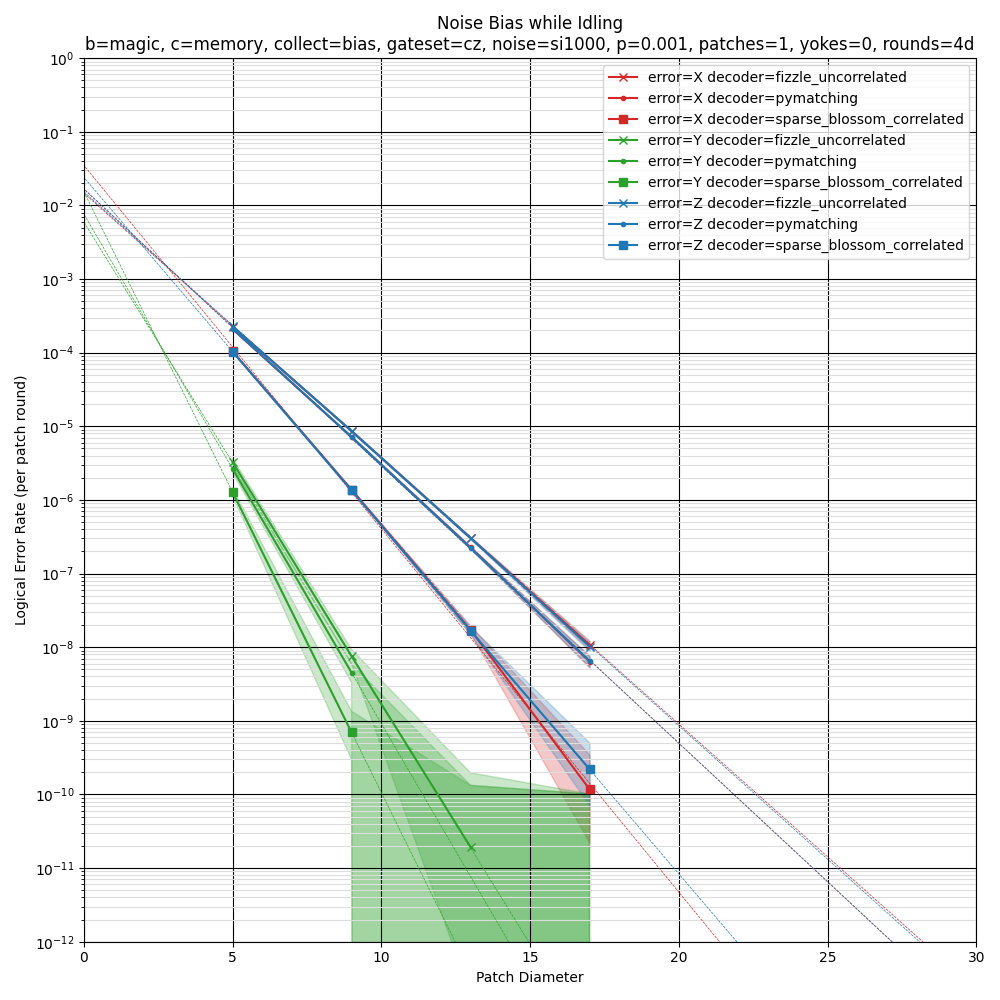
\includegraphics{assets/bias_memory.png}
        \hfill
        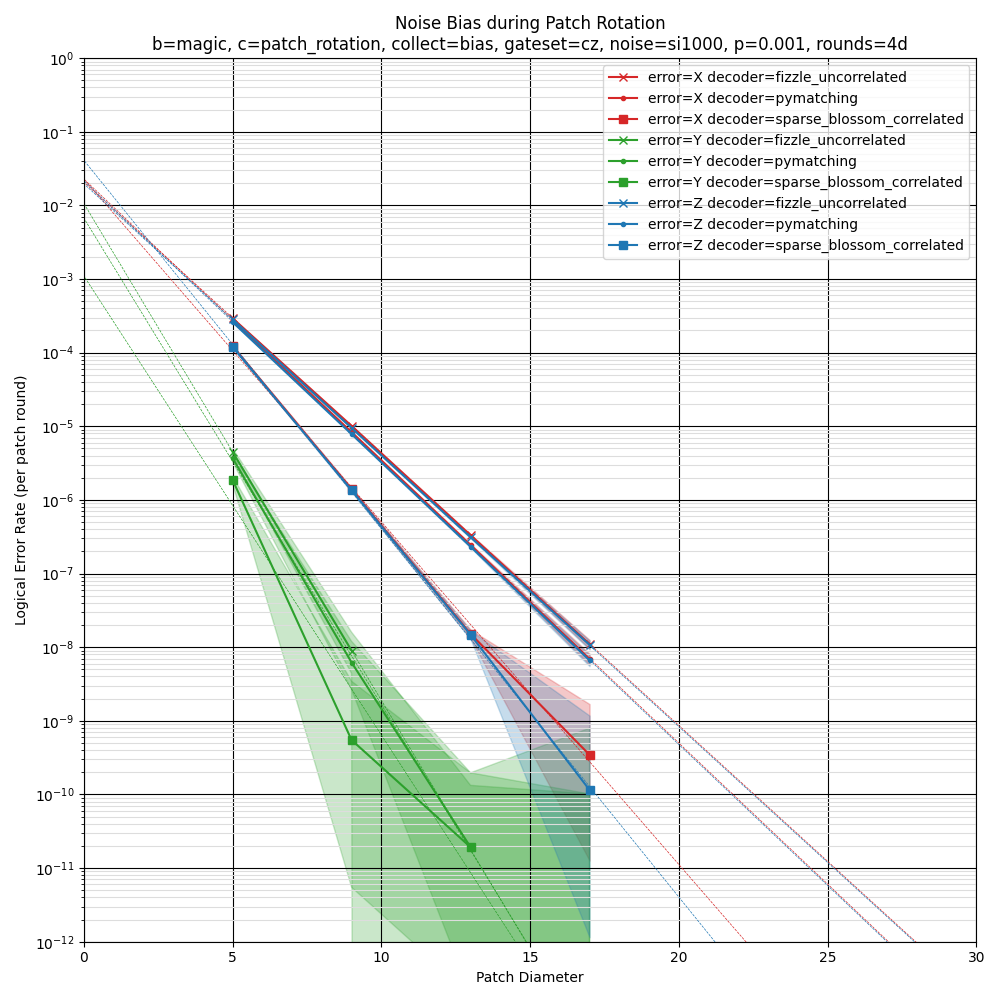
\includegraphics{assets/bias_patch_rotation.png}
    }
    \caption{
        Distribution of logical errors sampled from simulated surface code memory experiments (left) and patch rotation experiments (right).
        There is a strong bias away from Y type logical errors, with the Y error rate at a patch diameter of $d$ roughly matching the X or Z error rates at a patch diameter of $1.8d$.
        This bias occurs when using a union find decoder or a minimum weight perfect matching decoder, and when using uncorrelated decoding or correlated decoding.
        Shading indicates hypotheses with likelihoods within a factor of 1000 of the maximum likelihood hypothesis, given the sampled data.
    }
    \label{fig:bias}
\end{figure}

The second thing we were interested in quantifying by simulation was the distribution of complementary gaps, and whether or not the complementary gap was a good predictor of logical errors.
Originally, we were interested in these quantities because we expected them to be useful for understanding the size scaling of yoked qubits.
Ultimately, we ended up using different arguments to understand their scaling, but we still believe it should be possible to derive the scaling from the gap distribution.
Regardless, we haven't seen the gap distribution reported elsewhere and we expect it to be of independent interest.

To compute the gap distribution, we used pymatching's ``return\_weights'' feature.
We created circuits describing single surface code patches idling for $4d$ or $12d$ rounds.
The decoder's task was to predict whether the $X$ observable was flipped, and also whether the $Z$ observable was flipped.
Whether or not they both flipped (i.e. whether the $Y$ observable flipped) was revealed to the decoder, as a detector.
We had pymatching decode each shot with this detector both excited and not excited, allowing us to compute the gap and also (by picking the matching with the lower weight) the prediction it would have made without being told whether the $Y$ observable flipped.

We show the resulting distribution of gaps in \fig{gap}, and the logical error rate bucketed by gap in \fig{gap_calibration}.
These figures give two useful insights:
(1) extrapolating to larger numbers of rounds by taking the minimum of multiple samples from the gap distribution of a smaller number of rounds works well,
and (2) treating the gap as a log odds value is amazingly well calibrated as a predictor of whether a logical error has occurred.
It's likely also useful to know the general shape of gap distributions, though we haven't yet found a simple curve that fits the shape using realistic parameters.
There is a slight tendency for the gap to overestimate the chance of error, but the amount of overestimation appears to be consistent across patch diameters and round counts and so could be corrected by multiplying the gap by $0.9$.

\begin{figure}[h]
    \centering
    \resizebox{\linewidth}{!}{
        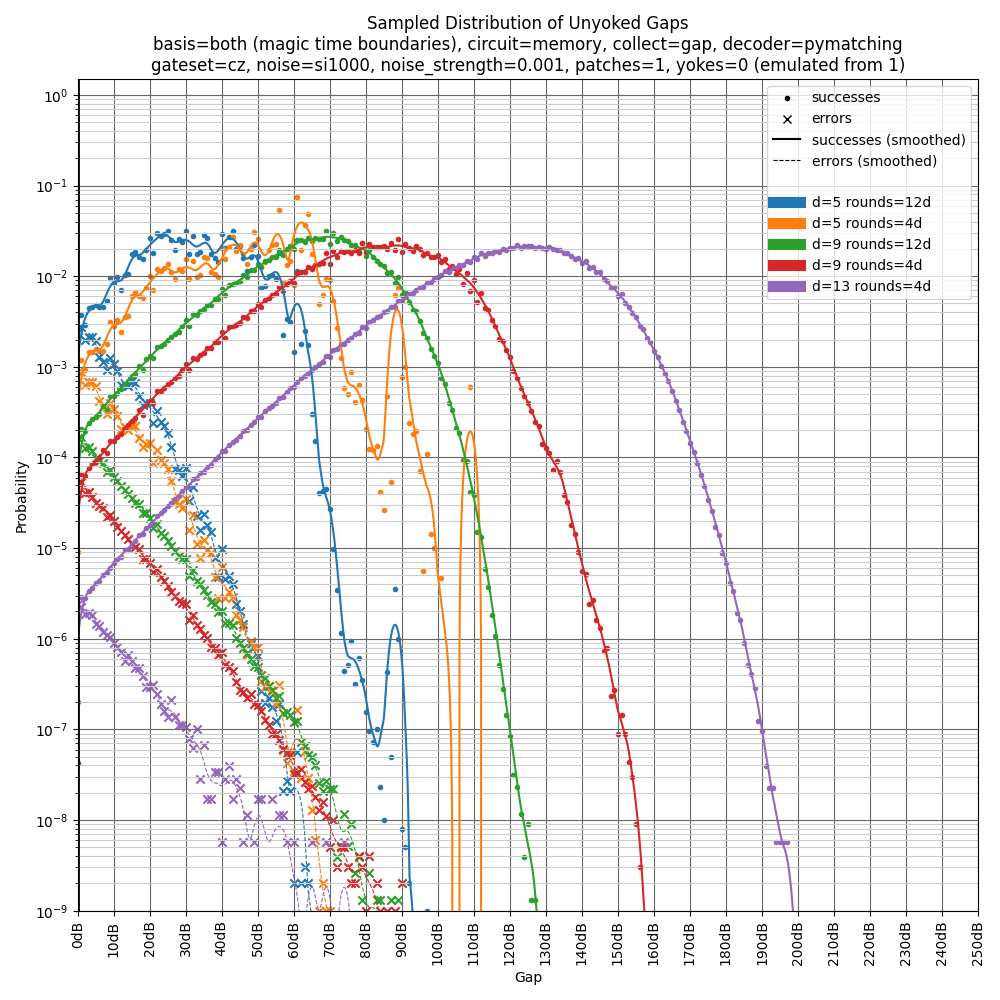
\includegraphics{assets/gap_distribution.png}
        \hfill
        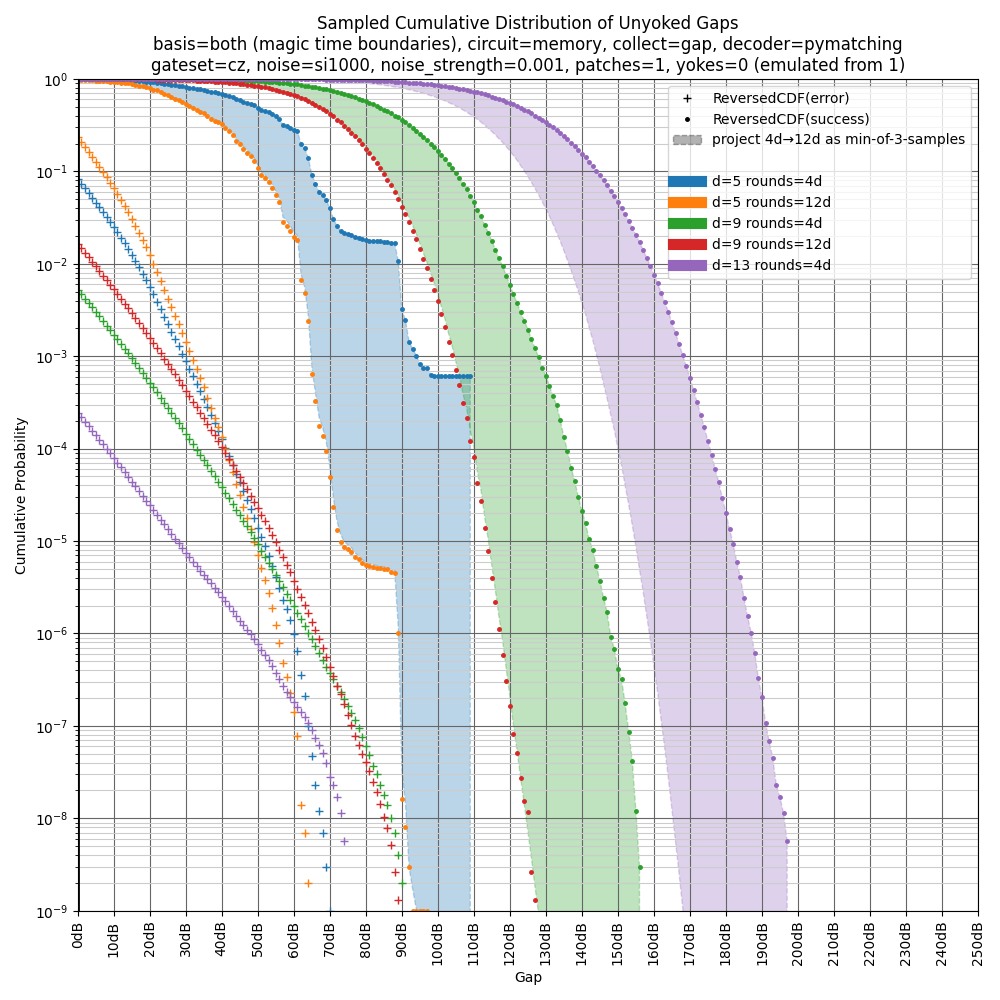
\includegraphics{assets/gap_cdf_extrapolation.png}
    }
    \caption{
        Distribution of sampled complementary gaps.
        Left: probability distributions smoothed by convolving with a cosine window and rescaling so that the smoothed output has the same area under the curve as the input.
        Right: cumulative distributions with extrapolations.
        Shaded areas show extrapolations.
        Each shaded area is bounded on one side by the points it is being extrapolated from (which have the same color) and on the other side by the extrapolation.
        Although a shaded area may appear to be bounded by points of a different color, this is not because those points are being used to define the shaded area, but rather because those points are sampling what is being extrapolated and the extrapolation is very good.
    }
    \label{fig:gap}
\end{figure}

\begin{figure}[h]
    \centering
    \resizebox{0.7\linewidth}{!}{
        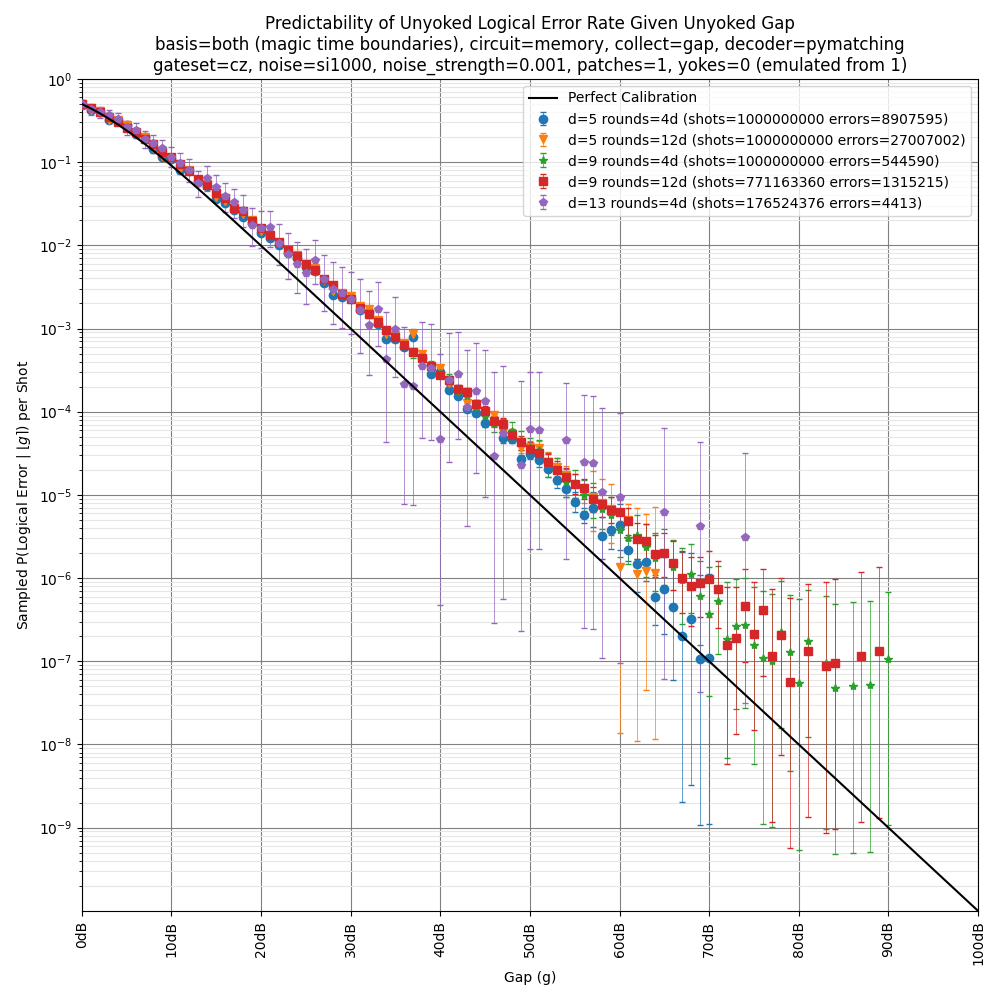
\includegraphics{assets/gap_calibration.png}
    }
    \caption{
        Sampled logical error rate conditioned on the gap.
        The perfect calibration line is $p_L = (1 + 10^{g/10})^{-1}$, where the logical error rate $p_L$ is produced by treating the gap $g$ as a log odds value in decibels and converting it to a probability.
        This plot shows that treating the gap as a log odds value produces a surprisingly well calibrated prediction for whether a logical error occurred, with a tendency towards underestimating the chance of error.
    }
    \label{fig:gap_calibration}
\end{figure}

The third thing we simulated is the core numerical result of this paper: the performance of yoked and unyoked memory experiments.
Our goal was to confirm that the yoked experiments had the scaling relationships we expected, and then to use those scaling relationships to extrapolate to practical sizes.
In \fig{scaling_laws_focus} we show specific examples of the expected asymptotic scaling relationships holding.
We used the numbers from those figures to create heuristic equations that predict the logical error rate from the number of rounds, the number of patches, and the number of yokes.
In \fig{scaling_laws_general} we show these equations in action, comparing the sampled logical error rates to the extrapolated logical error rates predicted by the equations.
We see good agreement between the two, despite the simplicity of the heuristic equations.

Our last numerical figure uses the heuristic equations to estimate footprints at sizes larger than we could simulate.
These estimates are shown in \fig{footprint}, for various target logical error rates.
This figure is the source of the ``2/3 physical qubits at $10^{-9}$ target error'' claim in the abstract of the paper.
As can be seen in the figure, the benefits improve slightly as the target logical error rate is lowered.


\begin{figure}[h]
    \centering
    \resizebox{\linewidth}{!}{
        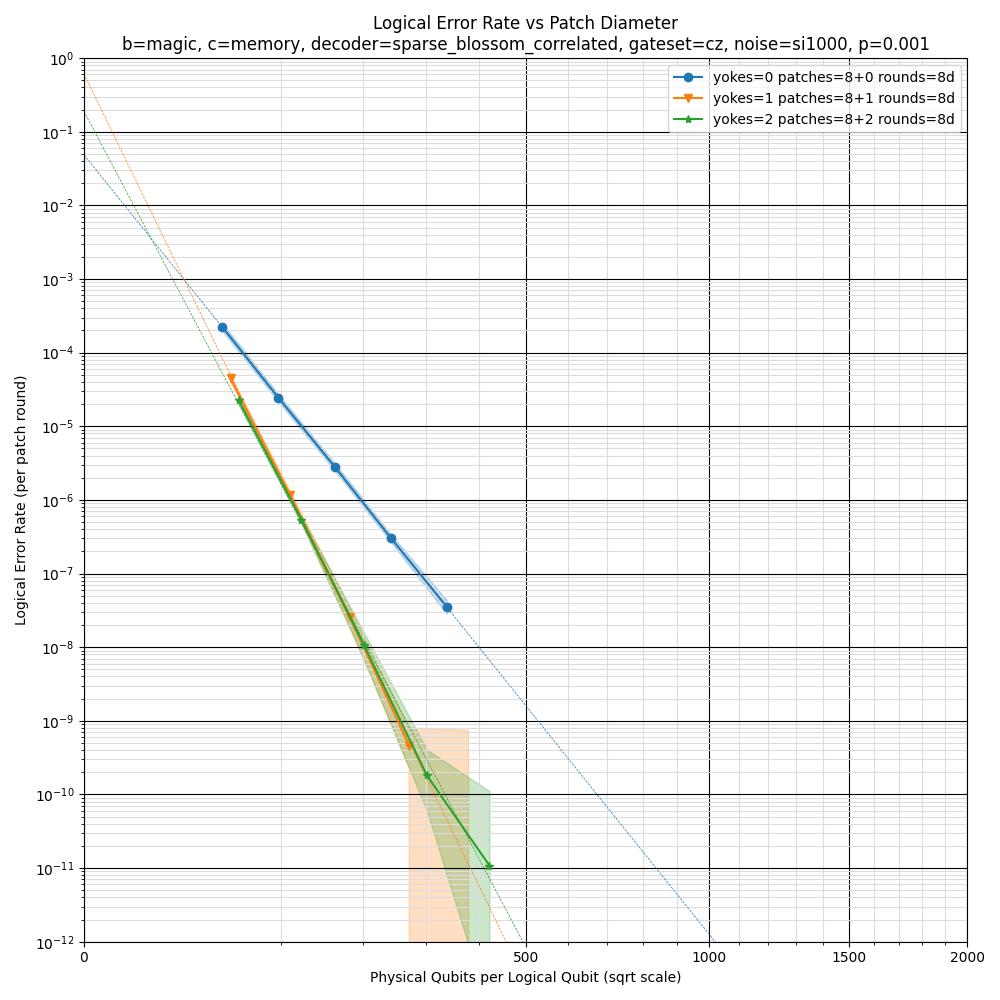
\includegraphics{assets/errors_yoked_memory_L=8_r=8d.png}
        \hfill
        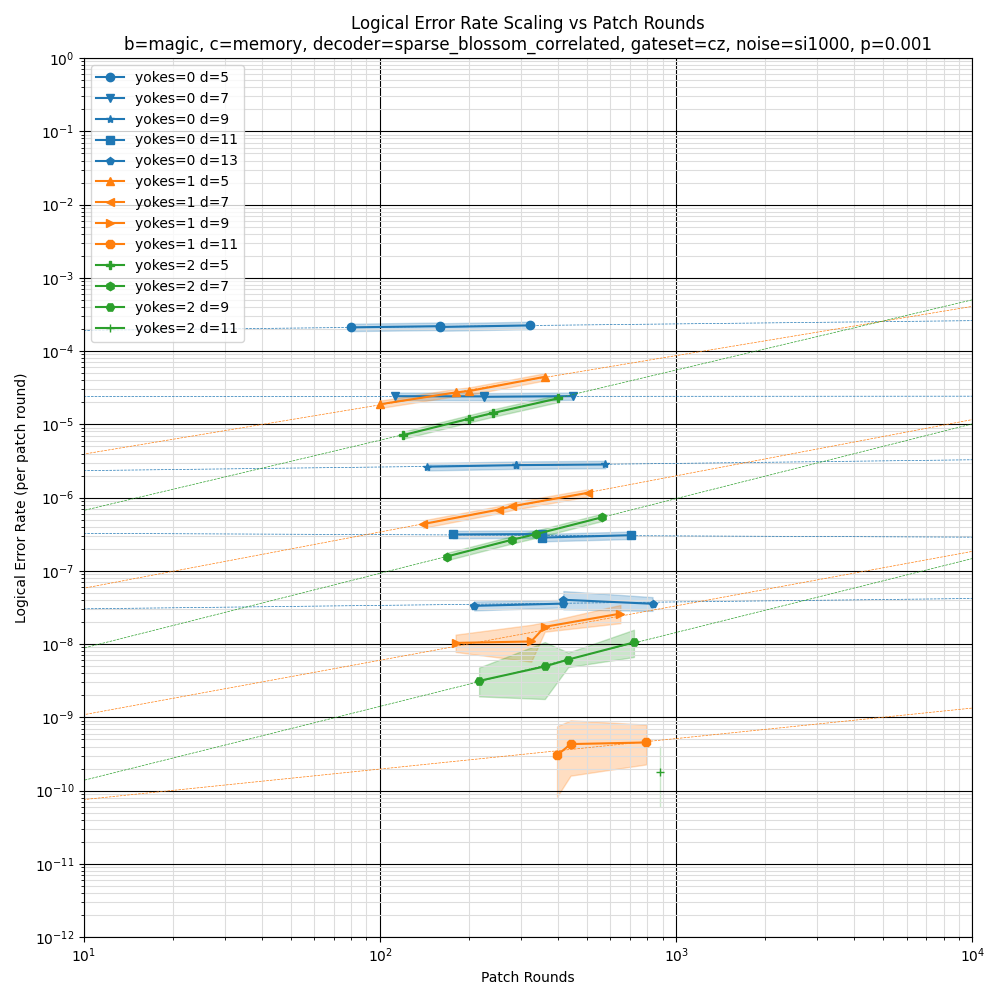
\includegraphics{assets/errors_yoked_memory_scaling.png}
    }
    \caption{
        Sampled logical error rates from simulations of yoked and unyoked surface code memory experiments.
        The left pane focuses on the largest case that was simulated, with $r=8d$ and $n=8$, showing how its logical error rate is exponentially suppressed versus patch diameter.
        The right pane shows all simulated cases where at least 10 errors were seen.
        The blue curves on the right are flat because they have error rates that scale linearly versus patch count $n$ and round count $r$.
        The yellow and green curves are sloped because they have error rates that scale approximately quadratically versus $n$ and $r$.
        Shading indicates hypotheses with likelihoods within a factor of 1000 of the maximum likelihood hypothesis, given the sampled data.
    }
    \label{fig:scaling_laws_focus}
\end{figure}

\begin{figure}[h]
    \centering
    \resizebox{0.7\linewidth}{!}{
        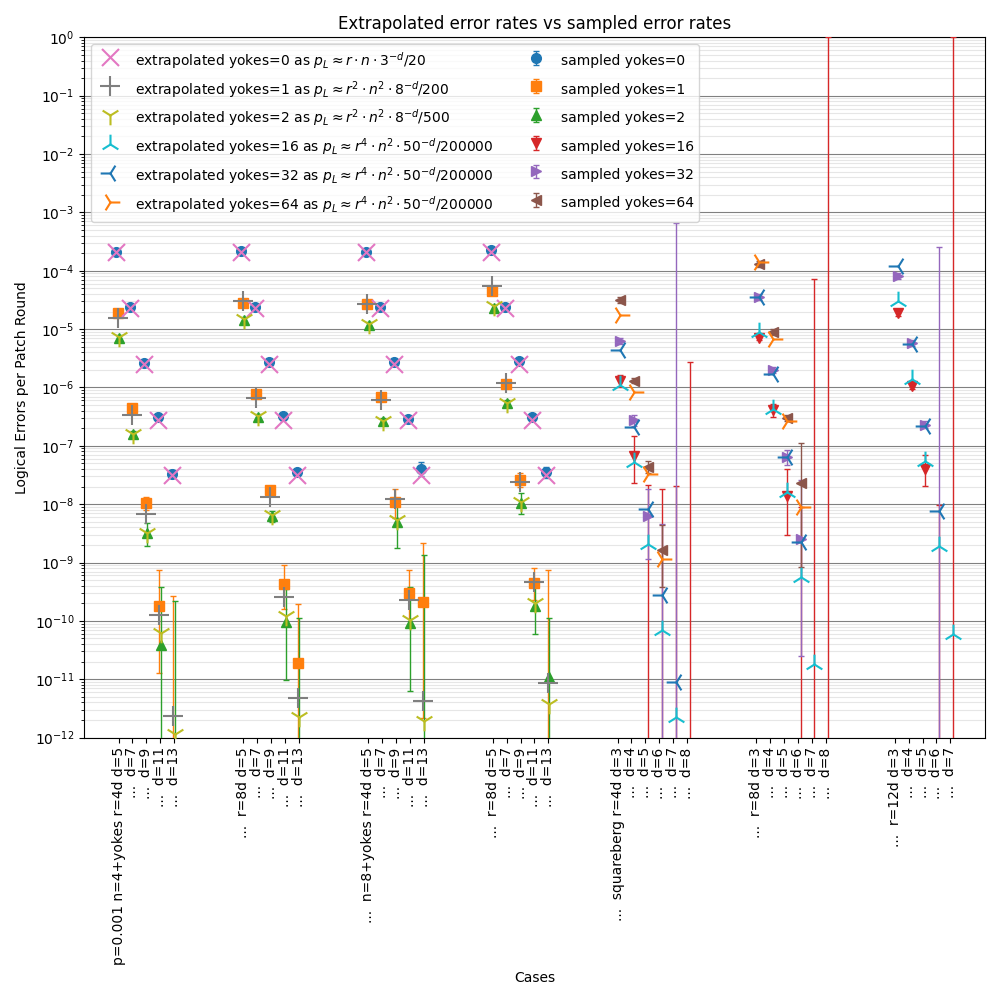
\includegraphics{assets/extrapolations.png}
    }
    \caption{
        The sampled logical error rates of all simulated cases, combined with heuristic equations that approximate them.
        Note that the heuristic formulas are specific to the noise model we used and to the noise strength of $p=0.001$.
        In the heuristic equations, we expect the number raised to the $-d$ to be proportional to $p$, but haven't done simulations to confirm this.
        Error bars indicate hypotheses with likelihoods within a factor of 1000 of the maximum likelihood hypothesis, given the sampled data.
    }
    \label{fig:scaling_laws_general}
\end{figure}

\begin{figure}[h]
    \centering
    \resizebox{\linewidth}{!}{
        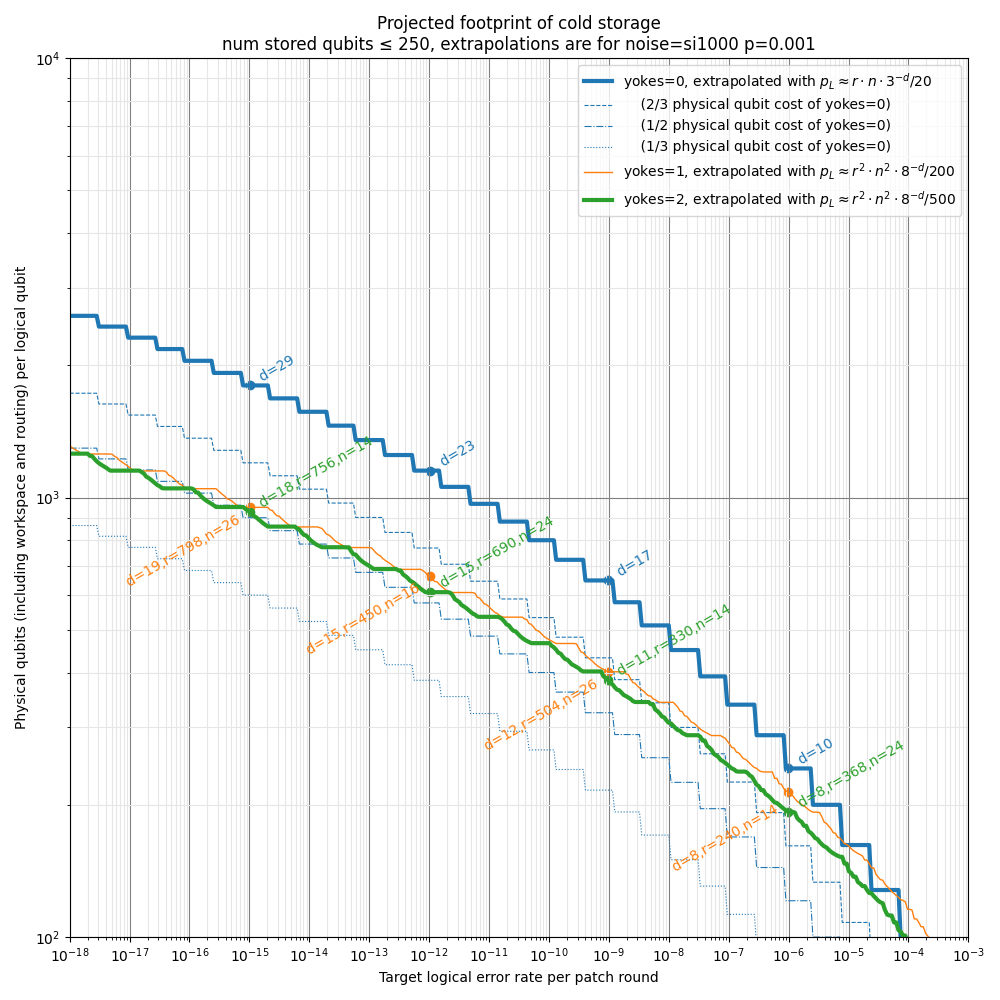
\includegraphics{assets/footprint_cold.png}
        \hfill
        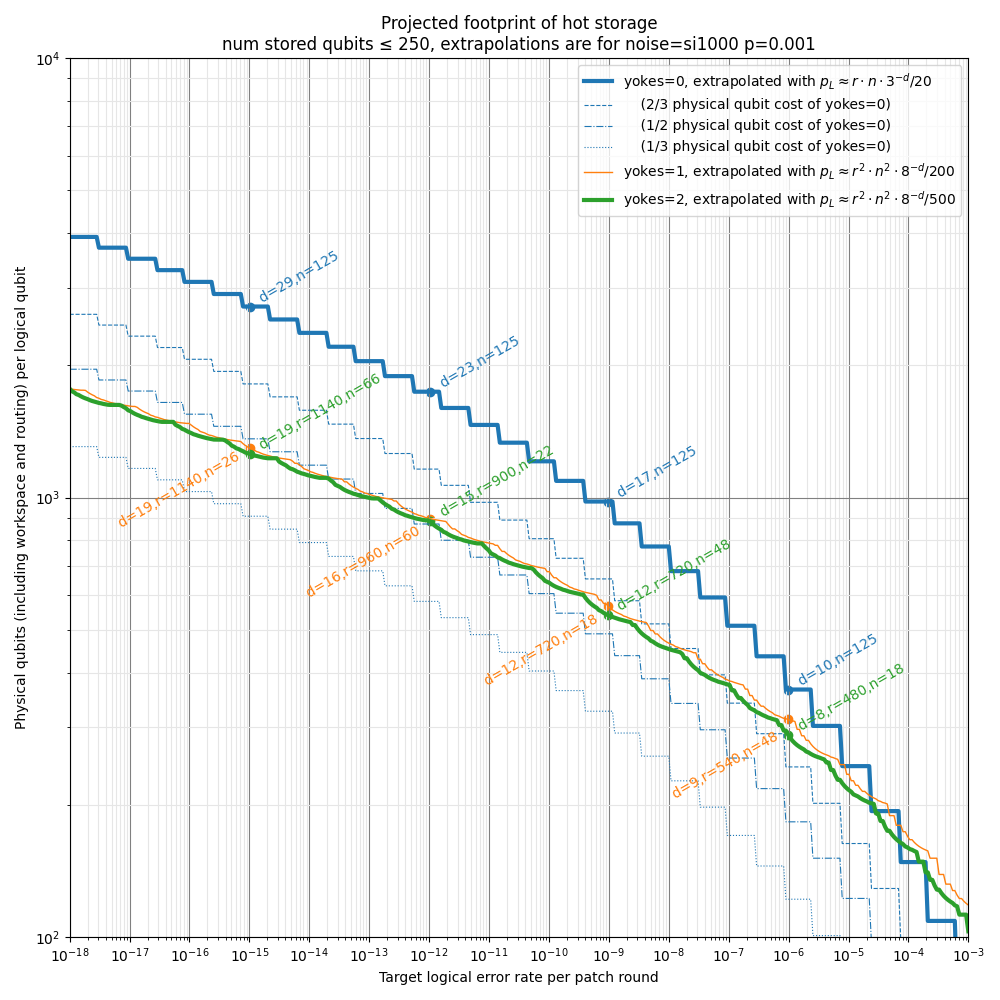
\includegraphics{assets/footprint_hot.png}
    }
    \caption{
        Extrapolated footprints of yoked qubit layouts versus unyoked qubit layouts, including the workspace and access hallway overheads shown in \fig{storage}.
        Projections for cold storage are on the left, and projections for hot storage are on the right.
        For each target logical error rate, various patch diameters $d$ and patch group sizes $n$ are tried, and the most efficient that meets the requirements is chosen (by using the approximate logical error heuristics demonstrated in \fig{scaling_laws_general}).
        A patch of diameter $d$ is assumed to cover $2(d+1)^2$ physical qubits (the +1 leaves some buffer space for lattice surgery).
        The yoked hot storage estimates target an access hallway utilization of 20\%.
    }
    \label{fig:footprint}
\end{figure}


\section{Conclusion}
\label{sec:conclusion}


% 2) In the intro, one thing kind of missing is "how prevalent will yoked surface codes be?" What size will they be and how often will my logical qubits live in patch sizes of 15 vs. 23, etc.? Just roughly giving a sense of this would be nice.

% 3) I still think the analogy in EC of the single parity bit used in a classical RAM might be nice to mention.

% 4) I think the complementary gap citation might be wrong? I think it's https://arxiv.org/abs/1302.2669

% 5) A bit confused by the yoke=2 label.

% 6) Maybe related: there's not much discussion of using the Yberg vs. iceberg codes. Do we have an idea of how much difference it makes? This would be relevant to how effective this strategy would be when employed with the color code.

% 7) Nit: re the latent soft information comments in the conclusion - I would expect every code has latent soft information. The real advantage here is that you can trick matching into activating that info. Just my two cents.

In this paper, we described how to ``yoke'' surface codes and estimated that yoked surface codes are 2/3 the size of normal surface codes, at reasonable target logical error rates.
Reducing the quantity of qubits required by surface codes is extremely useful, because the required quantity of physical qubits is the worst aspect of the surface code.

We considered two yoking codes: Yberg codes and iceberg codes.
We expected Yberg codes to create leaner yokes than iceberg codes, because Yberg codes have 1 stabilizer instead of 2.
Our results showed that this wasn't the case.
The lattice surgery for Yberg yokes is slightly more complex, requiring an ancillary lane, and this cancels out the potential advantage.
Although we think our most interesting result is that one extra stabilizer check can reduce the cost of surface codes by 30\%, in most situations doing the two iceberg stabilizer checks is the easier option.

Although in this paper we've only discussed the surface code, yoking should generalize to other topological codes.
For example, the honeycomb code~\cite{hastings2021dynamically,gidney2022honeycombplanar} likely has the same gap information and the same bias against one of the logical error types, and so should have essentially identical benefits from yoking.
The color code should also have gap information, and so should benefit from yoking (though not from the Yberg code since the color code lacks an anti-Y bias).
More generally, any code with solid soft information on whether the decoder's correction is correct is a reasonable candidate for yoking.

Stepping back, we notice that a key detail that makes yoking work has also appeared in other recent constructions~\cite{berthusen2023partialmeasure,lessbaconmorethreshold2023}: large stabilizers are measured less often than small stabilizers.
This is obvious in hindsight, but attempting to measure large stabilizers as often as small stabilizers can have disastrous results (where the small stabilizers could have been getting useful work done but instead are left waiting for the large stabilizers).
This is a potential loophole in proofs bounding the performance of quantum error correction.
If a proof implicitly assumes stabilizers are always measured together, then measuring large stabilizers less often could bypass the proof.



\section{Contributions}

Cody Jones had the initial idea of concatenating a $Y^{\otimes n}$ stabilizer over the surface code to double the code distance.
Craig Gidney got very excited by the idea and did all the work, exactly as Cody planned.
Michael Newman then asked ``what about second yoking?'' and Craig said that wouldn't work and Mike said ``but what if it did?'' and Craig got very excited until it all fell apart when figuring out the lattice surgery.

\section{Acknowledgements}

We thank Matt McEwen for useful and interesting discussions.
We thank the Google Quantum AI team for creating an environment where this work was possible.

\printbibliography

\appendix
\clearpage
\section{Noise Model}
\label{app:noise}

Simulations in this paper were done using the superconducting-inspired circuit noise model defined in \tab{noise_model}.
The name ``SI1000'' is short for Superconducting Inspired with 1000 nanosecond cycle.

\begin{table}[h]
    \centering
    \begin{tabular}{|r|l|}
    \hline
    Noise channel & Probability distribution of effects
    \\
    \hline
    $\text{MERR}_B(p)$ & $\begin{aligned}
        1-p &\rightarrow M_{B}
        \\
        p &\rightarrow M_{(-1 \cdot B)} \text{\;\;\;\;\;\emph{(i.e. measurement result is inverted)}}
    \end{aligned}$
    \\
    \hline
    $\text{XERR}(p)$ & $\begin{aligned}
        1-p &\rightarrow I
        \\
        p &\rightarrow X
    \end{aligned}$
    \\
    \hline
    $\text{ZERR}(p)$ & $\begin{aligned}
        1-p &\rightarrow I
        \\
        p &\rightarrow Z
    \end{aligned}$
    \\
    \hline
    $\text{DEP1}(p)$ & $\begin{aligned}
        1-p &\rightarrow I
        \\
        p/3 &\rightarrow X
        \\
        p/3 &\rightarrow Y
        \\
        p/3 &\rightarrow Z
    \end{aligned}$
    \\
    \hline
    $\text{DEP2}(p)$ & $\begin{aligned}
        1-p &\rightarrow I \otimes I
        &\;\;
        p/15 &\rightarrow I \otimes X
        &\;\;
        p/15 &\rightarrow I \otimes Y
        &\;\;
        p/15 &\rightarrow I \otimes Z
        \\
        p/15 &\rightarrow X \otimes I
        &\;\;
        p/15 &\rightarrow X \otimes X
        &\;\;
        p/15 &\rightarrow X \otimes Y
        &\;\;
        p/15 &\rightarrow X \otimes Z
        \\
        p/15 &\rightarrow Y \otimes I
        &\;\;
        p/15 &\rightarrow Y \otimes X
        &\;\;
        p/15 &\rightarrow Y \otimes Y
        &\;\;
        p/15 &\rightarrow Y \otimes Z
        \\
        p/15 &\rightarrow Z \otimes I
        &\;\;
        p/15 &\rightarrow Z \otimes X
        &\;\;
        p/15 &\rightarrow Z \otimes Y
        &\;\;
        p/15 &\rightarrow Z \otimes Z
    \end{aligned}$
    \\
    \hline
    \end{tabular}
    \caption{
        Definitions of various noise channels.
        Used by \tab{noise_model}.
    }
    \label{tab:noise_channels}
\end{table}

\begin{table}[h]
    \centering
    \begin{tabular}{|r|l|}
    \hline
    Ideal gate & Noisy replacement
    \\
    \hline
    (any single qubit unitary, including idling) $U_1$ & $\text{DEP1}(p / 10) \cdot U_1$
    \\
    $\text{CZ}$ & $\text{DEP2}(p) \cdot \text{CZ}$
    \\
    \hline
    $R_Z$ & $\text{XERR}(2p) \cdot R_Z$
    \\
    $M_Z$ & $\text{DEP1}(p) \cdot \text{MERR}_Z(5p)$
    \\
    \hline
    (Wait for $M_Z$ or $R_Z$) & $\text{DEP1}(2p)$
    \\
    \hline
    \end{tabular}
    \caption{
        The superconducting-inspired noise model ``SI1000'' used by simulations in this paper.
        The single parameter $p$ sets the two qubit gate error rate, with other error rates being relative to this rate.
        Measurements are noisiest while single qubit gates are least noisy.
        Qubits not being reset or measured during layers containing measurements or resets incur additional depolarization on top of other error mechanisms.
        Noise channels are defined in \tab{noise_channels}.
    }
    \label{tab:noise_model}
\end{table}

\clearpage
\section{Additional Data}
\label{app:additional_data}

\begin{figure}[h]
    \centering
    \resizebox{\linewidth}{!}{
        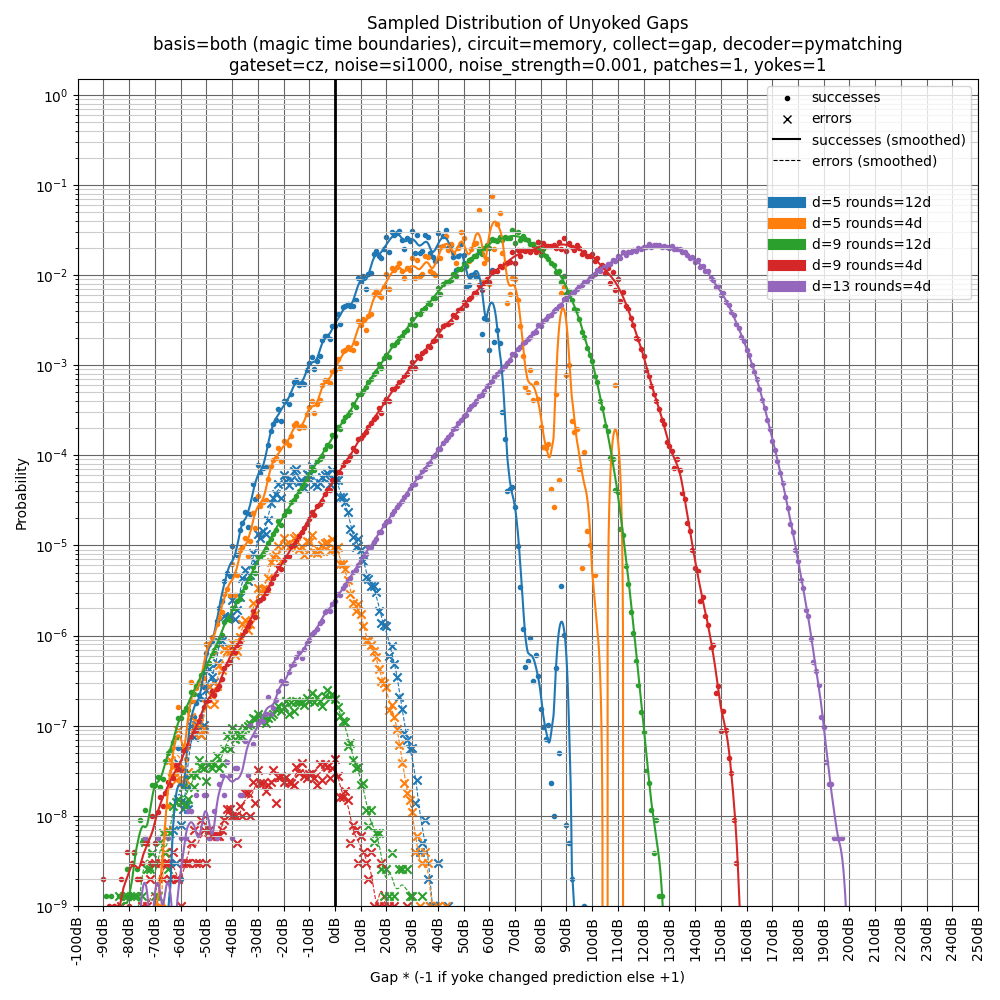
\includegraphics{assets/gap_distribution_yoked.png}
        \hfill
        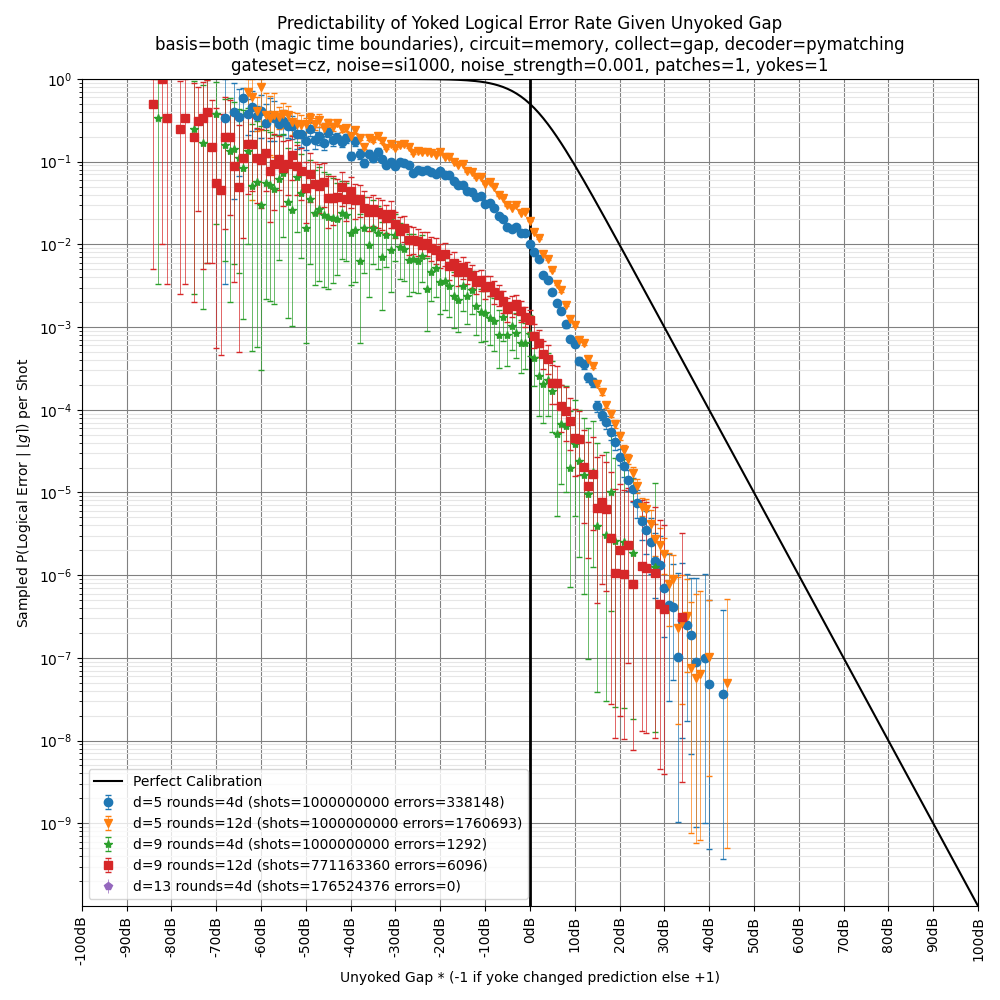
\includegraphics{assets/gap_calibration_yoked.png}
    }
    \caption{
        A variation of \fig{gap} and \fig{gap_calibration} with unyoked decoding replaced by yoked decoding (i.e. in these plots the decoder was told whether the $Y_L$ observable was flipped as it attempted to predict if $X_L$ and/or $Z_L$ were flipped).
        The gap is still computed without the yoke, but the sign of the gap is negated if the yoke made the decoder change its prediction.
        These plots show that yoking can improve error rates by orders of magnitude, and that the unyoked gap is still predictive of the logical error rate when using yoked decoding (but the prediction isn't well calibrated).
    }
    \label{fig:yoked_gap}
\end{figure}


\section{Nearly Double Yoking with Squareberg Codes}
\label{app:squareberg}

When we yoke a surface code using the boundary hugging trick, we can't use the trick again on the same boundary.
The boundary edges have already become normal edges; yoking at that location again would turn those normal edges into hyper edges not understood by matching-based decoders.
However, surface code patches have two boundaries of each type, which suggests the opportunity to attach more yokes as long as we attach them to different boundaries.
This allows us to use more complex yoking codes, as long as those codes satisfy the use-each-boundary-at-most-once constraint, which we'll call the ``2X2Z constraint''.
A code that satisfies the 2X2Z constraint has the property that an X error on any one qubit flips at most two stabilizers, and also that a Z error on any one qubit flips at most two stabilizers.
The 2X2Z constraint is sufficient to guarantee the code can be decoded by matching, independent of it being concatenated over the surface code.

Iceberg codes satisfy the 2X2Z constraint; in fact they are much stricter: each X and Z error only produces one symptom.
Given the fact that iceberg codes are only using half of the available constraint, a natural idea to try is to add more checks to the iceberg code or to use two interlocking iceberg codes.
For example, instead of including all qubits in a single X check, have row X checks and column X checks.
Row and column X checks would form a code with a Z-distance of 4.
We would like to also have an X-distance of 4, but there is a difficulty.
The Z checks can't also run along columns and rows, because the Z column checks would anticommute with the X row checks, and vice versa.
This can be solved by performing a partial transpose.

Consider an 8x8 grid, with 64 cells, where each cell is addressed by a 6-bit binary number.
The first three bits are the row bits, and the second three bits are the column bits.
We can specify a row, or column, as a bit string with wild cards.
For example, row 0 contains cells whose addresses match the pattern ``\texttt{000***}'' where ``\texttt{*}'' means wildcard.
Similarly, column 5 is matched by the pattern ``\texttt{***101}''.
From the perspective of these patterns, the reason that columns touch rows at exactly one location is that they have no wildcards in common and no fixed bits in common.
Analogously, the reason that two columns don't touch each other is that their patterns \emph{only} have wildcards in common.

If we rotate the column 5 pattern to the right by 1, we get the pattern ``\texttt{1***10}''.
Note that, versus any row pattern or column pattern, this pattern will have at least one wildcard in common.
This guarantees there will be an even number of cells matched by this pattern in that row or column.
It guarantees that a Z check using this pattern will commute with all the row X checks and all the column X checks.
We can do the same thing to all other column patterns and row patterns: rotate them to the right by 1, producing patterns with sets of matching cells that commute with the X checks if used as Z checks.
Furthermore, because bit-rotating addresses is a permutation, these Z checks will be isomorphic to the X checks.
They will also touch each qubit twice, and they will have an X-distance of 4.
These Z checks, together with the X checks, give us a distance 4 code satisfying the 2X2Z constraint.

The bit-rotation trick we just used will work on any $w \times h$ grid where $w$ and $h$ are multiples of 4.
We call the resulting family of $[[wh, (w-1)(h-1)+2, 4]]$ codes the ``squareberg codes''.
The $8 \times 8$ squareberg code is shown in \tab{squareberg_code}.

The error scaling of the squareberg code should be quadratic versus the number of patches $n$ and quartic versus the number of rounds $r$ between yoke checks.
The quadratic scaling versus $n$ is because undetectable logical errors correspond to four physical errors landing on the corners of a square within the grid.
There are $\Theta(n^2)$ of these squares.
The quartic scaling versus $r$ is because, when concatenated over the surface code, for a given choice of undetectable error square, each of the four errors at the corners of that square has $\Theta(r)$ times when it could occur.
Together they provide $\Theta(r^4)$ ways to fail.
In \fig{squareberg_potential} we confirm this $\Theta(n^2 r^4)$ scaling is reasonable, and use it to estimate costs at practical sizes.

The data in \fig{squareberg_potential} suggest that yoking with the $16 \times 16$ squareberg code would triple the coding rate of the surface code, at a target logical error rate per patch of $10^{-15}$ (this is roughly the target required for factoring 2048 bit numbers).
The reader may now be wondering why this is hidden away in an appendix, instead of the headline result of the paper.
The reason is that there is a major showstopping problem: we can't figure out how to compile the stabilizer checks into lattice surgery while satisfying the boundary hugging constraint, and therefore we don't currently know how to decode the construction to the necessary level of performance.
The sampled results in \fig{squareberg_potential} are only simulating idling, with magical measurement of the stabilizers instead of actual lattice surgery.
This is encouraging, but not definitive.
We've left this appendix in the paper, despite this issue, as encouragement to fix the remaining obstacles and claim the gains.

We also tried to make a two dimensional code involving Yberg-style checks, to complement the squareberg code, but weren't able to find a working construction.
Although doing Y row checks and Y column checks would achieve an X-distance and Z-distance of 4, the Y-distance would only be 1 and the anti-Y bias in the surface code isn't strong enough to compensate for a factor of 4 difference in the distance.
More annoyingly, the commutation constraint between stabilizers seems to interact badly with the 2X2Z constraint when Y-type stabilizers are present.
For example, consider a Y-type stabilizer touching a Z-type stabilizer.
They must touch at an even number of places, in order to commute.
At the places where they touch, no other stabilizer can have a Y or Z term because of the 2X2Z constraint.
Therefore a pair of X errors at two of the places where these stabilizers touch produces no symptoms, forcing either a small stabilizer or a distance 2 error mechanism into the code.

\begin{figure}[h]
    \centering
    \resizebox{\linewidth}{!}{
        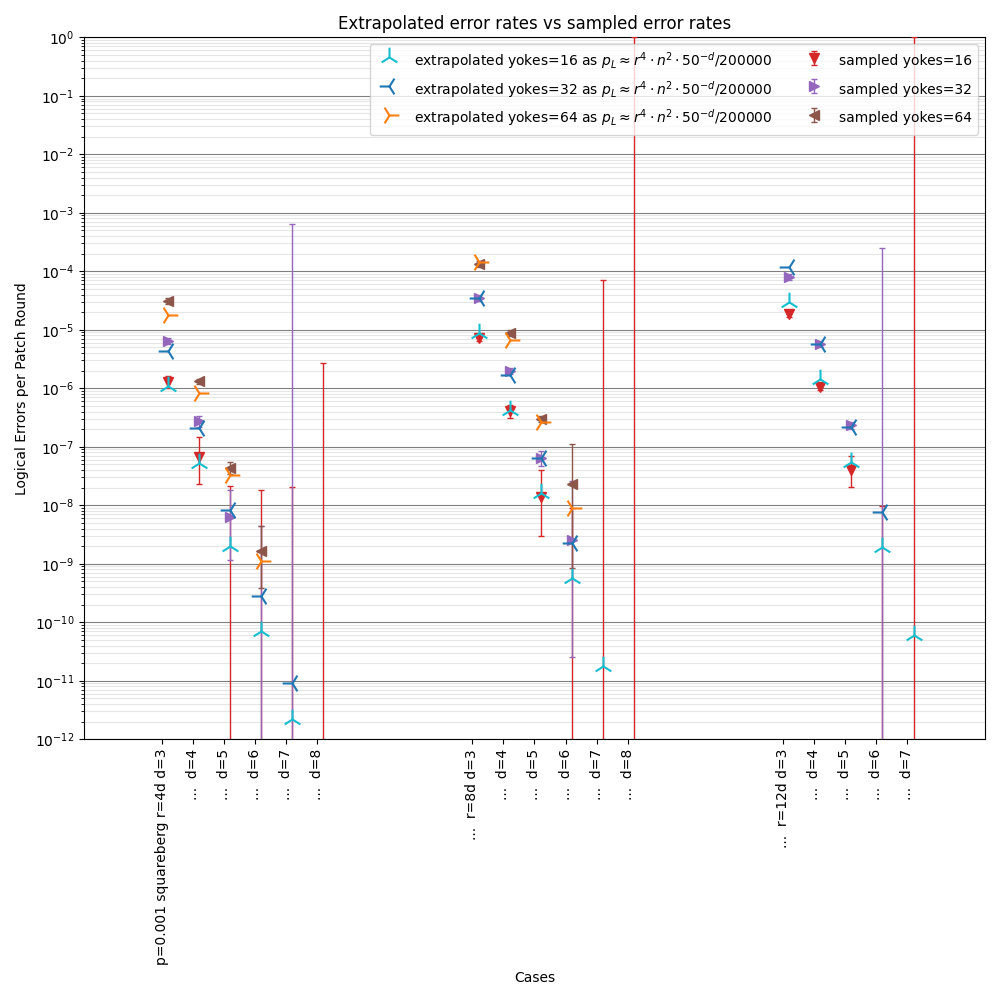
\includegraphics{assets/extrapolations_squareberg.png}
        \hfill
        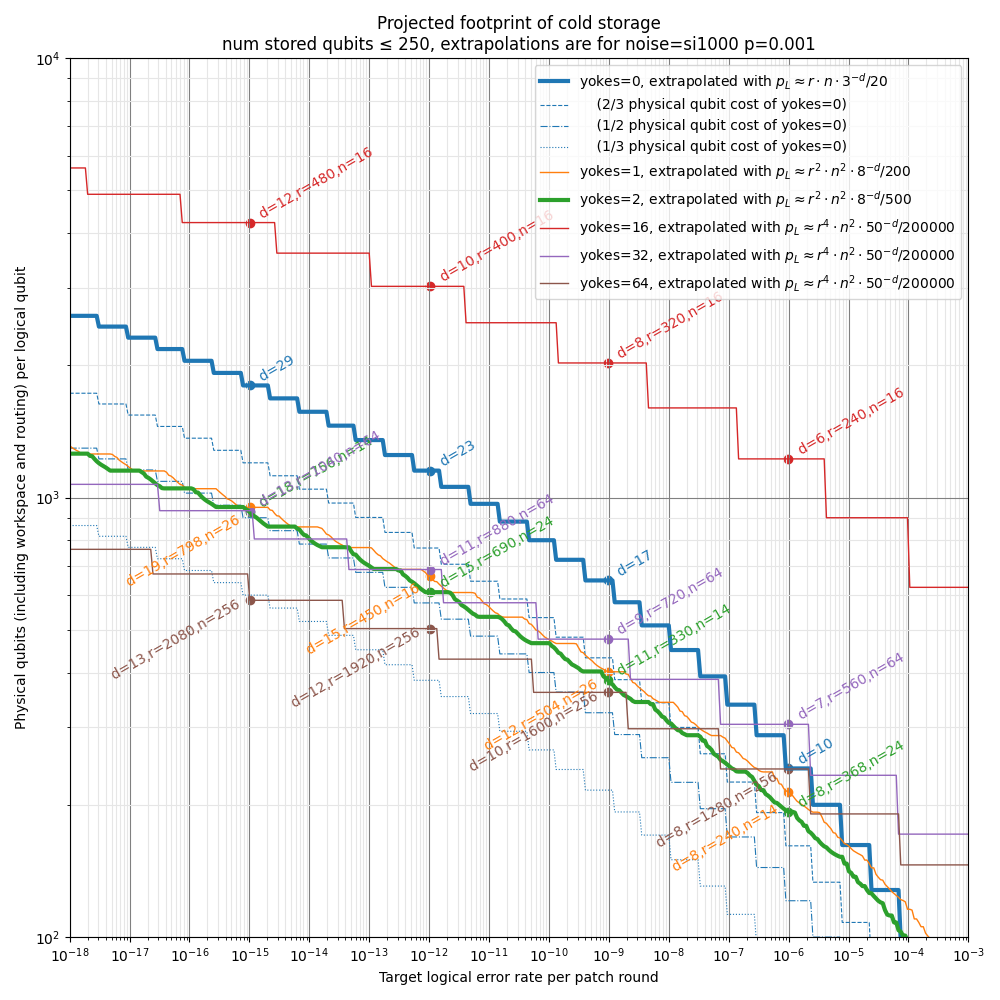
\includegraphics{assets/footprint_cold_squareberg.png}
    }
    \caption{
        Extrapolated costs of squareberg codes, showing a potential tripling of coding rate at a target patch error rate of $10^{-15}$.
        Achieving this would require compiling the squareberg yoked surface code into lattice surgery while satisfying the boundary hugging constraint, or writing a sufficiently performant decoder that didn't require the boundary hugging constraint in order to understand the decoding problem.
    }
    \label{fig:squareberg_potential}
\end{figure}

\begin{table}
    \centering
    \resizebox{\linewidth}{!}{
        \begin{tabular}{|c|c|c|c||c|c|c|c|c|c|c|c|}
\hline
\multicolumn{12}{|c|}{[[64, 34, 4]] Squareberg Code}
\\\hline
{\small X Col Checks} & {\small X Row Checks} & {\small Z Bi-Col Checks} & {\small Z Bi-Row Checks} & \multicolumn{8}{|c|}{Y Observables (positioned by location of Y term)}
\\\hline
\begin{tabular}{c}
    \texttt{X\_\_\_\_\_\_\_}\\
    \texttt{X\_\_\_\_\_\_\_}\\
    \texttt{X\_\_\_\_\_\_\_}\\
    \texttt{X\_\_\_\_\_\_\_}\\
    \texttt{X\_\_\_\_\_\_\_}\\
    \texttt{X\_\_\_\_\_\_\_}\\
    \texttt{X\_\_\_\_\_\_\_}\\
    \texttt{X\_\_\_\_\_\_\_}\\
\end{tabular}&\begin{tabular}{c}
    \texttt{XXXXXXXX}\\
    \texttt{\_\_\_\_\_\_\_\_}\\
    \texttt{\_\_\_\_\_\_\_\_}\\
    \texttt{\_\_\_\_\_\_\_\_}\\
    \texttt{\_\_\_\_\_\_\_\_}\\
    \texttt{\_\_\_\_\_\_\_\_}\\
    \texttt{\_\_\_\_\_\_\_\_}\\
    \texttt{\_\_\_\_\_\_\_\_}\\
\end{tabular}&\begin{tabular}{c}
    \texttt{ZZ\_\_\_\_\_\_}\\
    \texttt{\_\_\_\_\_\_\_\_}\\
    \texttt{ZZ\_\_\_\_\_\_}\\
    \texttt{\_\_\_\_\_\_\_\_}\\
    \texttt{ZZ\_\_\_\_\_\_}\\
    \texttt{\_\_\_\_\_\_\_\_}\\
    \texttt{ZZ\_\_\_\_\_\_}\\
    \texttt{\_\_\_\_\_\_\_\_}\\
\end{tabular}&\begin{tabular}{c}
    \texttt{Z\_Z\_Z\_Z\_}\\
    \texttt{Z\_Z\_Z\_Z\_}\\
    \texttt{\_\_\_\_\_\_\_\_}\\
    \texttt{\_\_\_\_\_\_\_\_}\\
    \texttt{\_\_\_\_\_\_\_\_}\\
    \texttt{\_\_\_\_\_\_\_\_}\\
    \texttt{\_\_\_\_\_\_\_\_}\\
    \texttt{\_\_\_\_\_\_\_\_}\\
\end{tabular}&\texttt{{\kern 5em}}&\texttt{{\kern 5em}}&\texttt{{\kern 5em}}&\texttt{{\kern 5em}}&\texttt{{\kern 5em}}&\texttt{{\kern 5em}}&\texttt{{\kern 5em}}&\texttt{{\kern 5em}}\\\hline
\begin{tabular}{c}
    \texttt{\_X\_\_\_\_\_\_}\\
    \texttt{\_X\_\_\_\_\_\_}\\
    \texttt{\_X\_\_\_\_\_\_}\\
    \texttt{\_X\_\_\_\_\_\_}\\
    \texttt{\_X\_\_\_\_\_\_}\\
    \texttt{\_X\_\_\_\_\_\_}\\
    \texttt{\_X\_\_\_\_\_\_}\\
    \texttt{\_X\_\_\_\_\_\_}\\
\end{tabular}&\begin{tabular}{c}
    \texttt{\_\_\_\_\_\_\_\_}\\
    \texttt{XXXXXXXX}\\
    \texttt{\_\_\_\_\_\_\_\_}\\
    \texttt{\_\_\_\_\_\_\_\_}\\
    \texttt{\_\_\_\_\_\_\_\_}\\
    \texttt{\_\_\_\_\_\_\_\_}\\
    \texttt{\_\_\_\_\_\_\_\_}\\
    \texttt{\_\_\_\_\_\_\_\_}\\
\end{tabular}&\begin{tabular}{c}
    \texttt{\_\_ZZ\_\_\_\_}\\
    \texttt{\_\_\_\_\_\_\_\_}\\
    \texttt{\_\_ZZ\_\_\_\_}\\
    \texttt{\_\_\_\_\_\_\_\_}\\
    \texttt{\_\_ZZ\_\_\_\_}\\
    \texttt{\_\_\_\_\_\_\_\_}\\
    \texttt{\_\_ZZ\_\_\_\_}\\
    \texttt{\_\_\_\_\_\_\_\_}\\
\end{tabular}&\begin{tabular}{c}
    \texttt{\_Z\_Z\_Z\_Z}\\
    \texttt{\_Z\_Z\_Z\_Z}\\
    \texttt{\_\_\_\_\_\_\_\_}\\
    \texttt{\_\_\_\_\_\_\_\_}\\
    \texttt{\_\_\_\_\_\_\_\_}\\
    \texttt{\_\_\_\_\_\_\_\_}\\
    \texttt{\_\_\_\_\_\_\_\_}\\
    \texttt{\_\_\_\_\_\_\_\_}\\
\end{tabular}&\texttt{{\kern 5em}}&\begin{tabular}{c}
    \texttt{ZZ\_\_\_\_\_\_}\\
    \texttt{ZY\_\_\_\_\_X}\\
    \texttt{\_\_\_\_\_\_\_\_}\\
    \texttt{\_\_\_\_\_\_\_\_}\\
    \texttt{\_\_\_\_\_\_\_\_}\\
    \texttt{\_\_\_\_\_\_\_\_}\\
    \texttt{\_\_\_\_\_\_\_\_}\\
    \texttt{\_X\_\_\_\_\_X}\\
\end{tabular}&\begin{tabular}{c}
    \texttt{Z\_Z\_\_\_\_\_}\\
    \texttt{Z\_Y\_\_\_X\_}\\
    \texttt{\_\_\_\_\_\_\_\_}\\
    \texttt{\_\_\_\_\_\_\_\_}\\
    \texttt{\_\_\_\_\_\_\_\_}\\
    \texttt{\_\_\_\_\_\_\_\_}\\
    \texttt{\_\_\_\_\_\_\_\_}\\
    \texttt{\_\_\_X\_\_\_X}\\
\end{tabular}&\begin{tabular}{c}
    \texttt{Z\_\_Z\_\_\_\_}\\
    \texttt{Z\_\_Y\_\_\_X}\\
    \texttt{\_\_\_\_\_\_\_\_}\\
    \texttt{\_\_\_\_\_\_\_\_}\\
    \texttt{\_\_\_\_\_\_\_\_}\\
    \texttt{\_\_\_\_\_\_\_\_}\\
    \texttt{\_\_\_\_\_\_\_\_}\\
    \texttt{\_\_\_X\_\_\_X}\\
\end{tabular}&\begin{tabular}{c}
    \texttt{Z\_\_\_Z\_\_\_}\\
    \texttt{Z\_\_\_Y\_X\_}\\
    \texttt{\_\_\_\_\_\_\_\_}\\
    \texttt{\_\_\_\_\_\_\_\_}\\
    \texttt{\_\_\_\_\_\_\_\_}\\
    \texttt{\_\_\_\_\_\_\_\_}\\
    \texttt{\_\_\_\_\_\_\_\_}\\
    \texttt{\_\_\_\_\_X\_X}\\
\end{tabular}&\begin{tabular}{c}
    \texttt{Z\_\_\_\_Z\_\_}\\
    \texttt{Z\_\_\_\_Y\_X}\\
    \texttt{\_\_\_\_\_\_\_\_}\\
    \texttt{\_\_\_\_\_\_\_\_}\\
    \texttt{\_\_\_\_\_\_\_\_}\\
    \texttt{\_\_\_\_\_\_\_\_}\\
    \texttt{\_\_\_\_\_\_\_\_}\\
    \texttt{\_\_\_\_\_X\_X}\\
\end{tabular}&\texttt{{\kern 5em}}&\texttt{{\kern 5em}}\\\hline
\begin{tabular}{c}
    \texttt{\_\_X\_\_\_\_\_}\\
    \texttt{\_\_X\_\_\_\_\_}\\
    \texttt{\_\_X\_\_\_\_\_}\\
    \texttt{\_\_X\_\_\_\_\_}\\
    \texttt{\_\_X\_\_\_\_\_}\\
    \texttt{\_\_X\_\_\_\_\_}\\
    \texttt{\_\_X\_\_\_\_\_}\\
    \texttt{\_\_X\_\_\_\_\_}\\
\end{tabular}&\begin{tabular}{c}
    \texttt{\_\_\_\_\_\_\_\_}\\
    \texttt{\_\_\_\_\_\_\_\_}\\
    \texttt{XXXXXXXX}\\
    \texttt{\_\_\_\_\_\_\_\_}\\
    \texttt{\_\_\_\_\_\_\_\_}\\
    \texttt{\_\_\_\_\_\_\_\_}\\
    \texttt{\_\_\_\_\_\_\_\_}\\
    \texttt{\_\_\_\_\_\_\_\_}\\
\end{tabular}&\begin{tabular}{c}
    \texttt{\_\_\_\_ZZ\_\_}\\
    \texttt{\_\_\_\_\_\_\_\_}\\
    \texttt{\_\_\_\_ZZ\_\_}\\
    \texttt{\_\_\_\_\_\_\_\_}\\
    \texttt{\_\_\_\_ZZ\_\_}\\
    \texttt{\_\_\_\_\_\_\_\_}\\
    \texttt{\_\_\_\_ZZ\_\_}\\
    \texttt{\_\_\_\_\_\_\_\_}\\
\end{tabular}&\begin{tabular}{c}
    \texttt{\_\_\_\_\_\_\_\_}\\
    \texttt{\_\_\_\_\_\_\_\_}\\
    \texttt{Z\_Z\_Z\_Z\_}\\
    \texttt{Z\_Z\_Z\_Z\_}\\
    \texttt{\_\_\_\_\_\_\_\_}\\
    \texttt{\_\_\_\_\_\_\_\_}\\
    \texttt{\_\_\_\_\_\_\_\_}\\
    \texttt{\_\_\_\_\_\_\_\_}\\
\end{tabular}&\texttt{{\kern 5em}}&\begin{tabular}{c}
    \texttt{ZZ\_\_\_\_\_\_}\\
    \texttt{\_\_\_\_\_\_\_\_}\\
    \texttt{ZY\_\_\_\_\_\_}\\
    \texttt{\_\_\_\_\_\_\_X}\\
    \texttt{\_\_\_\_\_\_\_\_}\\
    \texttt{\_\_\_\_\_\_\_\_}\\
    \texttt{\_X\_\_\_\_\_\_}\\
    \texttt{\_\_\_\_\_\_\_X}\\
\end{tabular}&\begin{tabular}{c}
    \texttt{Z\_Z\_\_\_\_\_}\\
    \texttt{\_\_\_\_\_\_\_\_}\\
    \texttt{Z\_Y\_\_\_\_\_}\\
    \texttt{\_\_\_\_\_\_X\_}\\
    \texttt{\_\_\_\_\_\_\_\_}\\
    \texttt{\_\_\_\_\_\_\_\_}\\
    \texttt{\_\_\_X\_\_\_\_}\\
    \texttt{\_\_\_\_\_\_\_X}\\
\end{tabular}&\begin{tabular}{c}
    \texttt{Z\_\_Z\_\_\_\_}\\
    \texttt{\_\_\_\_\_\_\_\_}\\
    \texttt{Z\_\_Y\_\_\_\_}\\
    \texttt{\_\_\_\_\_\_\_X}\\
    \texttt{\_\_\_\_\_\_\_\_}\\
    \texttt{\_\_\_\_\_\_\_\_}\\
    \texttt{\_\_\_X\_\_\_\_}\\
    \texttt{\_\_\_\_\_\_\_X}\\
\end{tabular}&\begin{tabular}{c}
    \texttt{Z\_\_\_Z\_\_\_}\\
    \texttt{\_\_\_\_\_\_\_\_}\\
    \texttt{Z\_\_\_Y\_\_\_}\\
    \texttt{\_\_\_\_\_\_X\_}\\
    \texttt{\_\_\_\_\_\_\_\_}\\
    \texttt{\_\_\_\_\_\_\_\_}\\
    \texttt{\_\_\_\_\_X\_\_}\\
    \texttt{\_\_\_\_\_\_\_X}\\
\end{tabular}&\begin{tabular}{c}
    \texttt{Z\_\_\_\_Z\_\_}\\
    \texttt{\_\_\_\_\_\_\_\_}\\
    \texttt{Z\_\_\_\_Y\_\_}\\
    \texttt{\_\_\_\_\_\_\_X}\\
    \texttt{\_\_\_\_\_\_\_\_}\\
    \texttt{\_\_\_\_\_\_\_\_}\\
    \texttt{\_\_\_\_\_X\_\_}\\
    \texttt{\_\_\_\_\_\_\_X}\\
\end{tabular}&\begin{tabular}{c}
    \texttt{Z\_\_\_\_\_Z\_}\\
    \texttt{\_\_\_\_\_\_\_\_}\\
    \texttt{Z\_\_\_\_\_Y\_}\\
    \texttt{\_\_\_\_\_\_X\_}\\
    \texttt{\_\_\_\_\_\_\_\_}\\
    \texttt{\_\_\_\_\_\_\_\_}\\
    \texttt{\_\_\_\_\_\_\_X}\\
    \texttt{\_\_\_\_\_\_\_X}\\
\end{tabular}&\begin{tabular}{c}
    \texttt{Z\_\_\_\_\_\_Z}\\
    \texttt{\_\_\_\_\_\_\_\_}\\
    \texttt{Z\_\_\_\_\_\_Y}\\
    \texttt{\_\_\_\_\_\_\_X}\\
    \texttt{\_\_\_\_\_\_\_\_}\\
    \texttt{\_\_\_\_\_\_\_\_}\\
    \texttt{\_\_\_\_\_\_\_X}\\
    \texttt{\_\_\_\_\_\_\_X}\\
\end{tabular}\\\hline
\begin{tabular}{c}
    \texttt{\_\_\_X\_\_\_\_}\\
    \texttt{\_\_\_X\_\_\_\_}\\
    \texttt{\_\_\_X\_\_\_\_}\\
    \texttt{\_\_\_X\_\_\_\_}\\
    \texttt{\_\_\_X\_\_\_\_}\\
    \texttt{\_\_\_X\_\_\_\_}\\
    \texttt{\_\_\_X\_\_\_\_}\\
    \texttt{\_\_\_X\_\_\_\_}\\
\end{tabular}&\begin{tabular}{c}
    \texttt{\_\_\_\_\_\_\_\_}\\
    \texttt{\_\_\_\_\_\_\_\_}\\
    \texttt{\_\_\_\_\_\_\_\_}\\
    \texttt{XXXXXXXX}\\
    \texttt{\_\_\_\_\_\_\_\_}\\
    \texttt{\_\_\_\_\_\_\_\_}\\
    \texttt{\_\_\_\_\_\_\_\_}\\
    \texttt{\_\_\_\_\_\_\_\_}\\
\end{tabular}&\begin{tabular}{c}
    \texttt{\_\_\_\_\_\_ZZ}\\
    \texttt{\_\_\_\_\_\_\_\_}\\
    \texttt{\_\_\_\_\_\_ZZ}\\
    \texttt{\_\_\_\_\_\_\_\_}\\
    \texttt{\_\_\_\_\_\_ZZ}\\
    \texttt{\_\_\_\_\_\_\_\_}\\
    \texttt{\_\_\_\_\_\_ZZ}\\
    \texttt{\_\_\_\_\_\_\_\_}\\
\end{tabular}&\begin{tabular}{c}
    \texttt{\_\_\_\_\_\_\_\_}\\
    \texttt{\_\_\_\_\_\_\_\_}\\
    \texttt{\_Z\_Z\_Z\_Z}\\
    \texttt{\_Z\_Z\_Z\_Z}\\
    \texttt{\_\_\_\_\_\_\_\_}\\
    \texttt{\_\_\_\_\_\_\_\_}\\
    \texttt{\_\_\_\_\_\_\_\_}\\
    \texttt{\_\_\_\_\_\_\_\_}\\
\end{tabular}&\texttt{{\kern 5em}}&\begin{tabular}{c}
    \texttt{ZZ\_\_\_\_\_\_}\\
    \texttt{\_\_\_\_\_\_\_\_}\\
    \texttt{\_\_\_\_\_\_\_\_}\\
    \texttt{ZY\_\_\_\_\_X}\\
    \texttt{\_\_\_\_\_\_\_\_}\\
    \texttt{\_\_\_\_\_\_\_\_}\\
    \texttt{\_\_\_\_\_\_\_\_}\\
    \texttt{\_X\_\_\_\_\_X}\\
\end{tabular}&\begin{tabular}{c}
    \texttt{Z\_Z\_\_\_\_\_}\\
    \texttt{\_\_\_\_\_\_\_\_}\\
    \texttt{\_\_\_\_\_\_\_\_}\\
    \texttt{Z\_Y\_\_\_X\_}\\
    \texttt{\_\_\_\_\_\_\_\_}\\
    \texttt{\_\_\_\_\_\_\_\_}\\
    \texttt{\_\_\_\_\_\_\_\_}\\
    \texttt{\_\_\_X\_\_\_X}\\
\end{tabular}&\begin{tabular}{c}
    \texttt{Z\_\_Z\_\_\_\_}\\
    \texttt{\_\_\_\_\_\_\_\_}\\
    \texttt{\_\_\_\_\_\_\_\_}\\
    \texttt{Z\_\_Y\_\_\_X}\\
    \texttt{\_\_\_\_\_\_\_\_}\\
    \texttt{\_\_\_\_\_\_\_\_}\\
    \texttt{\_\_\_\_\_\_\_\_}\\
    \texttt{\_\_\_X\_\_\_X}\\
\end{tabular}&\begin{tabular}{c}
    \texttt{Z\_\_\_Z\_\_\_}\\
    \texttt{\_\_\_\_\_\_\_\_}\\
    \texttt{\_\_\_\_\_\_\_\_}\\
    \texttt{Z\_\_\_Y\_X\_}\\
    \texttt{\_\_\_\_\_\_\_\_}\\
    \texttt{\_\_\_\_\_\_\_\_}\\
    \texttt{\_\_\_\_\_\_\_\_}\\
    \texttt{\_\_\_\_\_X\_X}\\
\end{tabular}&\begin{tabular}{c}
    \texttt{Z\_\_\_\_Z\_\_}\\
    \texttt{\_\_\_\_\_\_\_\_}\\
    \texttt{\_\_\_\_\_\_\_\_}\\
    \texttt{Z\_\_\_\_Y\_X}\\
    \texttt{\_\_\_\_\_\_\_\_}\\
    \texttt{\_\_\_\_\_\_\_\_}\\
    \texttt{\_\_\_\_\_\_\_\_}\\
    \texttt{\_\_\_\_\_X\_X}\\
\end{tabular}&\texttt{{\kern 5em}}&\texttt{{\kern 5em}}\\\hline
\begin{tabular}{c}
    \texttt{\_\_\_\_X\_\_\_}\\
    \texttt{\_\_\_\_X\_\_\_}\\
    \texttt{\_\_\_\_X\_\_\_}\\
    \texttt{\_\_\_\_X\_\_\_}\\
    \texttt{\_\_\_\_X\_\_\_}\\
    \texttt{\_\_\_\_X\_\_\_}\\
    \texttt{\_\_\_\_X\_\_\_}\\
    \texttt{\_\_\_\_X\_\_\_}\\
\end{tabular}&\begin{tabular}{c}
    \texttt{\_\_\_\_\_\_\_\_}\\
    \texttt{\_\_\_\_\_\_\_\_}\\
    \texttt{\_\_\_\_\_\_\_\_}\\
    \texttt{\_\_\_\_\_\_\_\_}\\
    \texttt{XXXXXXXX}\\
    \texttt{\_\_\_\_\_\_\_\_}\\
    \texttt{\_\_\_\_\_\_\_\_}\\
    \texttt{\_\_\_\_\_\_\_\_}\\
\end{tabular}&\begin{tabular}{c}
    \texttt{\_\_\_\_\_\_\_\_}\\
    \texttt{ZZ\_\_\_\_\_\_}\\
    \texttt{\_\_\_\_\_\_\_\_}\\
    \texttt{ZZ\_\_\_\_\_\_}\\
    \texttt{\_\_\_\_\_\_\_\_}\\
    \texttt{ZZ\_\_\_\_\_\_}\\
    \texttt{\_\_\_\_\_\_\_\_}\\
    \texttt{ZZ\_\_\_\_\_\_}\\
\end{tabular}&\begin{tabular}{c}
    \texttt{\_\_\_\_\_\_\_\_}\\
    \texttt{\_\_\_\_\_\_\_\_}\\
    \texttt{\_\_\_\_\_\_\_\_}\\
    \texttt{\_\_\_\_\_\_\_\_}\\
    \texttt{Z\_Z\_Z\_Z\_}\\
    \texttt{Z\_Z\_Z\_Z\_}\\
    \texttt{\_\_\_\_\_\_\_\_}\\
    \texttt{\_\_\_\_\_\_\_\_}\\
\end{tabular}&\texttt{{\kern 5em}}&\begin{tabular}{c}
    \texttt{ZZ\_\_\_\_\_\_}\\
    \texttt{\_\_\_\_\_\_\_\_}\\
    \texttt{\_\_\_\_\_\_\_\_}\\
    \texttt{\_\_\_\_\_\_\_\_}\\
    \texttt{ZY\_\_\_\_\_\_}\\
    \texttt{\_\_\_\_\_\_\_X}\\
    \texttt{\_X\_\_\_\_\_\_}\\
    \texttt{\_\_\_\_\_\_\_X}\\
\end{tabular}&\begin{tabular}{c}
    \texttt{Z\_Z\_\_\_\_\_}\\
    \texttt{\_\_\_\_\_\_\_\_}\\
    \texttt{\_\_\_\_\_\_\_\_}\\
    \texttt{\_\_\_\_\_\_\_\_}\\
    \texttt{Z\_Y\_\_\_\_\_}\\
    \texttt{\_\_\_\_\_\_X\_}\\
    \texttt{\_\_\_X\_\_\_\_}\\
    \texttt{\_\_\_\_\_\_\_X}\\
\end{tabular}&\begin{tabular}{c}
    \texttt{Z\_\_Z\_\_\_\_}\\
    \texttt{\_\_\_\_\_\_\_\_}\\
    \texttt{\_\_\_\_\_\_\_\_}\\
    \texttt{\_\_\_\_\_\_\_\_}\\
    \texttt{Z\_\_Y\_\_\_\_}\\
    \texttt{\_\_\_\_\_\_\_X}\\
    \texttt{\_\_\_X\_\_\_\_}\\
    \texttt{\_\_\_\_\_\_\_X}\\
\end{tabular}&\begin{tabular}{c}
    \texttt{Z\_\_\_Z\_\_\_}\\
    \texttt{\_\_\_\_\_\_\_\_}\\
    \texttt{\_\_\_\_\_\_\_\_}\\
    \texttt{\_\_\_\_\_\_\_\_}\\
    \texttt{Z\_\_\_Y\_\_\_}\\
    \texttt{\_\_\_\_\_\_X\_}\\
    \texttt{\_\_\_\_\_X\_\_}\\
    \texttt{\_\_\_\_\_\_\_X}\\
\end{tabular}&\begin{tabular}{c}
    \texttt{Z\_\_\_\_Z\_\_}\\
    \texttt{\_\_\_\_\_\_\_\_}\\
    \texttt{\_\_\_\_\_\_\_\_}\\
    \texttt{\_\_\_\_\_\_\_\_}\\
    \texttt{Z\_\_\_\_Y\_\_}\\
    \texttt{\_\_\_\_\_\_\_X}\\
    \texttt{\_\_\_\_\_X\_\_}\\
    \texttt{\_\_\_\_\_\_\_X}\\
\end{tabular}&\begin{tabular}{c}
    \texttt{Z\_\_\_\_\_Z\_}\\
    \texttt{\_\_\_\_\_\_\_\_}\\
    \texttt{\_\_\_\_\_\_\_\_}\\
    \texttt{\_\_\_\_\_\_\_\_}\\
    \texttt{Z\_\_\_\_\_Y\_}\\
    \texttt{\_\_\_\_\_\_X\_}\\
    \texttt{\_\_\_\_\_\_\_X}\\
    \texttt{\_\_\_\_\_\_\_X}\\
\end{tabular}&\begin{tabular}{c}
    \texttt{Z\_\_\_\_\_\_Z}\\
    \texttt{\_\_\_\_\_\_\_\_}\\
    \texttt{\_\_\_\_\_\_\_\_}\\
    \texttt{\_\_\_\_\_\_\_\_}\\
    \texttt{Z\_\_\_\_\_\_Y}\\
    \texttt{\_\_\_\_\_\_\_X}\\
    \texttt{\_\_\_\_\_\_\_X}\\
    \texttt{\_\_\_\_\_\_\_X}\\
\end{tabular}\\\hline
\begin{tabular}{c}
    \texttt{\_\_\_\_\_X\_\_}\\
    \texttt{\_\_\_\_\_X\_\_}\\
    \texttt{\_\_\_\_\_X\_\_}\\
    \texttt{\_\_\_\_\_X\_\_}\\
    \texttt{\_\_\_\_\_X\_\_}\\
    \texttt{\_\_\_\_\_X\_\_}\\
    \texttt{\_\_\_\_\_X\_\_}\\
    \texttt{\_\_\_\_\_X\_\_}\\
\end{tabular}&\begin{tabular}{c}
    \texttt{\_\_\_\_\_\_\_\_}\\
    \texttt{\_\_\_\_\_\_\_\_}\\
    \texttt{\_\_\_\_\_\_\_\_}\\
    \texttt{\_\_\_\_\_\_\_\_}\\
    \texttt{\_\_\_\_\_\_\_\_}\\
    \texttt{XXXXXXXX}\\
    \texttt{\_\_\_\_\_\_\_\_}\\
    \texttt{\_\_\_\_\_\_\_\_}\\
\end{tabular}&\begin{tabular}{c}
    \texttt{\_\_\_\_\_\_\_\_}\\
    \texttt{\_\_ZZ\_\_\_\_}\\
    \texttt{\_\_\_\_\_\_\_\_}\\
    \texttt{\_\_ZZ\_\_\_\_}\\
    \texttt{\_\_\_\_\_\_\_\_}\\
    \texttt{\_\_ZZ\_\_\_\_}\\
    \texttt{\_\_\_\_\_\_\_\_}\\
    \texttt{\_\_ZZ\_\_\_\_}\\
\end{tabular}&\begin{tabular}{c}
    \texttt{\_\_\_\_\_\_\_\_}\\
    \texttt{\_\_\_\_\_\_\_\_}\\
    \texttt{\_\_\_\_\_\_\_\_}\\
    \texttt{\_\_\_\_\_\_\_\_}\\
    \texttt{\_Z\_Z\_Z\_Z}\\
    \texttt{\_Z\_Z\_Z\_Z}\\
    \texttt{\_\_\_\_\_\_\_\_}\\
    \texttt{\_\_\_\_\_\_\_\_}\\
\end{tabular}&\texttt{{\kern 5em}}&\begin{tabular}{c}
    \texttt{ZZ\_\_\_\_\_\_}\\
    \texttt{\_\_\_\_\_\_\_\_}\\
    \texttt{\_\_\_\_\_\_\_\_}\\
    \texttt{\_\_\_\_\_\_\_\_}\\
    \texttt{\_\_\_\_\_\_\_\_}\\
    \texttt{ZY\_\_\_\_\_X}\\
    \texttt{\_\_\_\_\_\_\_\_}\\
    \texttt{\_X\_\_\_\_\_X}\\
\end{tabular}&\begin{tabular}{c}
    \texttt{Z\_Z\_\_\_\_\_}\\
    \texttt{\_\_\_\_\_\_\_\_}\\
    \texttt{\_\_\_\_\_\_\_\_}\\
    \texttt{\_\_\_\_\_\_\_\_}\\
    \texttt{\_\_\_\_\_\_\_\_}\\
    \texttt{Z\_Y\_\_\_X\_}\\
    \texttt{\_\_\_\_\_\_\_\_}\\
    \texttt{\_\_\_X\_\_\_X}\\
\end{tabular}&\begin{tabular}{c}
    \texttt{Z\_\_Z\_\_\_\_}\\
    \texttt{\_\_\_\_\_\_\_\_}\\
    \texttt{\_\_\_\_\_\_\_\_}\\
    \texttt{\_\_\_\_\_\_\_\_}\\
    \texttt{\_\_\_\_\_\_\_\_}\\
    \texttt{Z\_\_Y\_\_\_X}\\
    \texttt{\_\_\_\_\_\_\_\_}\\
    \texttt{\_\_\_X\_\_\_X}\\
\end{tabular}&\begin{tabular}{c}
    \texttt{Z\_\_\_Z\_\_\_}\\
    \texttt{\_\_\_\_\_\_\_\_}\\
    \texttt{\_\_\_\_\_\_\_\_}\\
    \texttt{\_\_\_\_\_\_\_\_}\\
    \texttt{\_\_\_\_\_\_\_\_}\\
    \texttt{Z\_\_\_Y\_X\_}\\
    \texttt{\_\_\_\_\_\_\_\_}\\
    \texttt{\_\_\_\_\_X\_X}\\
\end{tabular}&\begin{tabular}{c}
    \texttt{Z\_\_\_\_Z\_\_}\\
    \texttt{\_\_\_\_\_\_\_\_}\\
    \texttt{\_\_\_\_\_\_\_\_}\\
    \texttt{\_\_\_\_\_\_\_\_}\\
    \texttt{\_\_\_\_\_\_\_\_}\\
    \texttt{Z\_\_\_\_Y\_X}\\
    \texttt{\_\_\_\_\_\_\_\_}\\
    \texttt{\_\_\_\_\_X\_X}\\
\end{tabular}&\texttt{{\kern 5em}}&\texttt{{\kern 5em}}\\\hline
\begin{tabular}{c}
    \texttt{\_\_\_\_\_\_X\_}\\
    \texttt{\_\_\_\_\_\_X\_}\\
    \texttt{\_\_\_\_\_\_X\_}\\
    \texttt{\_\_\_\_\_\_X\_}\\
    \texttt{\_\_\_\_\_\_X\_}\\
    \texttt{\_\_\_\_\_\_X\_}\\
    \texttt{\_\_\_\_\_\_X\_}\\
    \texttt{\_\_\_\_\_\_X\_}\\
\end{tabular}&\begin{tabular}{c}
    \texttt{\_\_\_\_\_\_\_\_}\\
    \texttt{\_\_\_\_\_\_\_\_}\\
    \texttt{\_\_\_\_\_\_\_\_}\\
    \texttt{\_\_\_\_\_\_\_\_}\\
    \texttt{\_\_\_\_\_\_\_\_}\\
    \texttt{\_\_\_\_\_\_\_\_}\\
    \texttt{XXXXXXXX}\\
    \texttt{\_\_\_\_\_\_\_\_}\\
\end{tabular}&\begin{tabular}{c}
    \texttt{\_\_\_\_\_\_\_\_}\\
    \texttt{\_\_\_\_ZZ\_\_}\\
    \texttt{\_\_\_\_\_\_\_\_}\\
    \texttt{\_\_\_\_ZZ\_\_}\\
    \texttt{\_\_\_\_\_\_\_\_}\\
    \texttt{\_\_\_\_ZZ\_\_}\\
    \texttt{\_\_\_\_\_\_\_\_}\\
    \texttt{\_\_\_\_ZZ\_\_}\\
\end{tabular}&\begin{tabular}{c}
    \texttt{\_\_\_\_\_\_\_\_}\\
    \texttt{\_\_\_\_\_\_\_\_}\\
    \texttt{\_\_\_\_\_\_\_\_}\\
    \texttt{\_\_\_\_\_\_\_\_}\\
    \texttt{\_\_\_\_\_\_\_\_}\\
    \texttt{\_\_\_\_\_\_\_\_}\\
    \texttt{Z\_Z\_Z\_Z\_}\\
    \texttt{Z\_Z\_Z\_Z\_}\\
\end{tabular}&\texttt{{\kern 5em}}&\texttt{{\kern 5em}}&\begin{tabular}{c}
    \texttt{Z\_Z\_\_\_\_\_}\\
    \texttt{\_\_\_\_\_\_\_\_}\\
    \texttt{\_\_\_\_\_\_\_\_}\\
    \texttt{\_\_\_\_\_\_\_\_}\\
    \texttt{\_\_\_\_\_\_\_\_}\\
    \texttt{\_\_\_\_\_\_\_\_}\\
    \texttt{Z\_YX\_\_\_\_}\\
    \texttt{\_\_\_\_\_\_XX}\\
\end{tabular}&\texttt{{\kern 5em}}&\begin{tabular}{c}
    \texttt{Z\_\_\_Z\_\_\_}\\
    \texttt{\_\_\_\_\_\_\_\_}\\
    \texttt{\_\_\_\_\_\_\_\_}\\
    \texttt{\_\_\_\_\_\_\_\_}\\
    \texttt{\_\_\_\_\_\_\_\_}\\
    \texttt{\_\_\_\_\_\_\_\_}\\
    \texttt{Z\_\_\_YX\_\_}\\
    \texttt{\_\_\_\_\_\_XX}\\
\end{tabular}&\texttt{{\kern 5em}}&\begin{tabular}{c}
    \texttt{Z\_\_\_\_\_Z\_}\\
    \texttt{\_\_\_\_\_\_\_\_}\\
    \texttt{\_\_\_\_\_\_\_\_}\\
    \texttt{\_\_\_\_\_\_\_\_}\\
    \texttt{\_\_\_\_\_\_\_\_}\\
    \texttt{\_\_\_\_\_\_\_\_}\\
    \texttt{Z\_\_\_\_\_YX}\\
    \texttt{\_\_\_\_\_\_XX}\\
\end{tabular}&\texttt{{\kern 5em}}\\\hline
\begin{tabular}{c}
    \texttt{\_\_\_\_\_\_\_X}\\
    \texttt{\_\_\_\_\_\_\_X}\\
    \texttt{\_\_\_\_\_\_\_X}\\
    \texttt{\_\_\_\_\_\_\_X}\\
    \texttt{\_\_\_\_\_\_\_X}\\
    \texttt{\_\_\_\_\_\_\_X}\\
    \texttt{\_\_\_\_\_\_\_X}\\
    \texttt{\_\_\_\_\_\_\_X}\\
\end{tabular}&\begin{tabular}{c}
    \texttt{\_\_\_\_\_\_\_\_}\\
    \texttt{\_\_\_\_\_\_\_\_}\\
    \texttt{\_\_\_\_\_\_\_\_}\\
    \texttt{\_\_\_\_\_\_\_\_}\\
    \texttt{\_\_\_\_\_\_\_\_}\\
    \texttt{\_\_\_\_\_\_\_\_}\\
    \texttt{\_\_\_\_\_\_\_\_}\\
    \texttt{XXXXXXXX}\\
\end{tabular}&\begin{tabular}{c}
    \texttt{\_\_\_\_\_\_\_\_}\\
    \texttt{\_\_\_\_\_\_ZZ}\\
    \texttt{\_\_\_\_\_\_\_\_}\\
    \texttt{\_\_\_\_\_\_ZZ}\\
    \texttt{\_\_\_\_\_\_\_\_}\\
    \texttt{\_\_\_\_\_\_ZZ}\\
    \texttt{\_\_\_\_\_\_\_\_}\\
    \texttt{\_\_\_\_\_\_ZZ}\\
\end{tabular}&\begin{tabular}{c}
    \texttt{\_\_\_\_\_\_\_\_}\\
    \texttt{\_\_\_\_\_\_\_\_}\\
    \texttt{\_\_\_\_\_\_\_\_}\\
    \texttt{\_\_\_\_\_\_\_\_}\\
    \texttt{\_\_\_\_\_\_\_\_}\\
    \texttt{\_\_\_\_\_\_\_\_}\\
    \texttt{\_Z\_Z\_Z\_Z}\\
    \texttt{\_Z\_Z\_Z\_Z}\\
\end{tabular}&\texttt{{\kern 5em}}&\texttt{{\kern 5em}}&\begin{tabular}{c}
    \texttt{Z\_Z\_\_\_\_\_}\\
    \texttt{\_\_\_\_\_\_\_\_}\\
    \texttt{\_\_\_\_\_\_\_\_}\\
    \texttt{\_\_\_\_\_\_\_\_}\\
    \texttt{\_\_\_\_\_\_\_\_}\\
    \texttt{\_\_\_\_\_\_\_\_}\\
    \texttt{\_\_\_\_\_\_\_\_}\\
    \texttt{Z\_YX\_\_XX}\\
\end{tabular}&\texttt{{\kern 5em}}&\begin{tabular}{c}
    \texttt{Z\_\_\_Z\_\_\_}\\
    \texttt{\_\_\_\_\_\_\_\_}\\
    \texttt{\_\_\_\_\_\_\_\_}\\
    \texttt{\_\_\_\_\_\_\_\_}\\
    \texttt{\_\_\_\_\_\_\_\_}\\
    \texttt{\_\_\_\_\_\_\_\_}\\
    \texttt{\_\_\_\_\_\_\_\_}\\
    \texttt{Z\_\_\_YXXX}\\
\end{tabular}&\texttt{{\kern 5em}}&\texttt{{\kern 5em}}&\texttt{{\kern 5em}}\\\hline
\end{tabular}

    }
    \caption{
        Definitions of stabilizers and observables in the $n=64,k=34,d=4$ squareberg code.
        Each cell shows the entries of a stabilizer or observable as an 8x8 grid of pauli terms; one term for each of the 64 physical qubits.
        Note that both the X observables and Z observables can be recovered from the Y observables, because the X observables contain no Y or Z terms and the Z observables contain no X or Y terms.
        Note that two of the listed checks are redundant (the product of all X col checks is equal to the product of all X row checks, and the product of all Z bi-col checks is equal to the product of all Z bi-row checks).
    }
    \label{tab:squareberg_code}
\end{table}

\end{document}
